\documentclass{book}

% document style
\usepackage[italian]{babel}
\usepackage[
  a4paper,
  bindingoffset=0in,
  left=1in,
  right=1in,
  top=1in,
  bottom=1in,
  footskip=.25in
]{geometry}

% references
\usepackage{hyperref}
\hypersetup{
  pdftitle={Appunti di Algoritmi e Prencipi dell'Informatica},
  pdfauthor={Fabio Vokrri},
  pdfsubject={Corso di Algoritmi e Prencipi dell'Informatica del professor Davide Martinenghi, Politecnico di Milano 2021-2022},
  pdfkeywords={Informatica Teorica, Strutture Dati, Algoritmi},  colorlinks=false,
  linkcolor=black,
  pdfpagemode=FullScreen,
}

% graphics and images
\usepackage{tikz}
\usetikzlibrary{automata, arrows.meta, positioning}

\usepackage{graphicx}
\graphicspath{ {../images/} }

% math
\usepackage{amsmath,amsfonts,amssymb,amsthm}

\newtheorem{theorem}{Teorema}[section]
\newtheorem{definition}{Definizione}[section]
\newtheorem{thesis}{Tesi}[section]

% coding style
\newcommand{\code}[1]{\lstinline[mathescape]{#1}}
\usepackage{listings}

\lstdefinestyle{mystyle}{
  basicstyle=\ttfamily,
  numberstyle=\tiny,
  breakatwhitespace=false,
  breaklines=true,
  captionpos=b,
  keepspaces=true,
  numbers=left,
  numbersep=7.5pt,
  showspaces=false,
  showstringspaces=false,
  showtabs=false,
  tabsize=2,
  xleftmargin=20pt,
  frame=l,
  aboveskip=10pt,
  belowskip=10pt,
  keywordstyle=\bf\itshape,
  classoffset=0,
  morekeywords={for, down, to, by, each, in, while, and, or, repeat, until, if, else, return, swap, with},
}

\lstset{style=mystyle}

\renewcommand\lstlistingname{codice}
\renewcommand\lstlistlistingname{codice}

% MAIN
\begin{document}

  \title{\Huge \textbf{Algoritmi e Principi dell'Informatica}}
\author{\huge Fabio Vokrri}

\begin{titlepage}
  \maketitle
\end{titlepage}

  \tableofcontents
  \clearpage

  \part{Informatica Teorica}

  \chapter{Complessità del Calcolo}
  Nei capitoli precedenti si è dimostrato come esistano alcuni problemi che, pur essendo ben definiti, non sono risolvibili algoritmicamente, per cui non esiste una TM in grado di risolvere quel determinato problema. Un'altra difficoltà da tenere in considerazione quando si manipolano i problemi, risiede nel tempo di esecuzione, ovvero il tempo impiegato dal programma per fornire una soluzione: se non è possibile ottenere una soluzione in un tempo ragionevole, ovviamente, il problema diventa intrattabile, nonostante sia teoricamente risolvibile.

  Il concetto di intrattabilità è strettamente correlato al concetto di complessità del calcolo: più il problema è complesso e meno questo diventa trattabile. Informalmente, la complessità indica una misura del prezzo da pagare per risolvere il problema. Le risorse che si utilizzano per la risoluzione di un problema sono principalmente due: lo spazio, ovvero la memoria necessaria all'algoritmo, e il tempo richiesto per produrre la soluzione. Si parlerà quindi di complessità spaziale e di complessità temporale.

  Si osservi inoltre che le due risorse, quella temporale e quella spaziale, seppur sembrino indipendenti l'una dall'altra, sono in realtà correlate: alla riduzione di utilizzo di una risorsa aumenta l'altra e viceversa. 

  \section{Analisi di complessità}
  La complessità del calcolo dipende dalla dimensione e, spesso, anche dai particolari valori assunti dai dati in ingresso. Per questo motivo, si rende necessario effettuare un'analisi del caso pessimo, del caso medio e del caso ottimo, in funzione della dimensione dei dati in ingresso. Più formalmente, tali casi rappresentano rispettivamente la scelta di ingressi per cui viene eseguito il massimo numero di istruzioni nel programma, il comportamento del programma in relazione alla possibile distribuzione dei dati e la scelta di input per cui viene eseguito il minor numero di istruzioni.

  In generale, il caso ottimo non è di particolare interesse e il caso medio richiede la conoscenza della distribuzione dei dati in ingresso (non sempre nota). Il caso pessimo, invece, è particolarmente interessante in quanto fornisce i peggiori risultati ottenibili dall'algoritmo in termini di consumo di spazio o tempo; si garantisce quindi che tutte le soluzioni proposte dall'algoritmo abbiano un dispendio di risorse minore rispetto al caso pessimo, indipendentemente dalla tipologia degli ingressi. Dunque, se il caso pessimo è ritenuto accettabile, allora anche tutti gli altri casi lo sono. 

  Inoltre, a differenza di quanto analizzato per la risolvibilità dei problemi, la complessità non è collegata solo al problema che si vuole affrontare, ma dipende anche dell'algoritmo che si utilizza per risolverlo. 

  \paragraph{}
  Nel capitolo sugli automi, è stato più volte affermato che le Macchine di Turing sono il formalismo più potente che si ha a disposizione per la risoluzione di problemi, dunque, risulta ragionevole definire la complessità temporale e spaziale impiegando un tale modello.

  \begin{definition} \label{complessita temporale} 
    Sia \(M\) una TM deterministica a \(k\) nastri e sia \(x\in I^*\). Sia \(c_0\vdash c_1\vdash....\vdash c_r\) una computazione, ovvero una sequenza di transizioni di \(M\) tale che \(c_0=<q_0,\;\!\uparrow\! x,\; \!\uparrow\! Z_0,\; ...,\; \!\uparrow\! Z_0>\) e \\ \(c_i=<q_i,\;x_i\!\uparrow\! y_i,\; \alpha_{i1}\!\uparrow\! \beta_{i1},\; ...,\; \alpha_{ik}\!\uparrow\! \beta_{ik}>\), in cui \(c_r\) è una configurazione di arresto, se esiste. Allora, la funzione che rappresenta la complessità temporale \({T}_M\) di \(M\) è definita nel seguente modo:
    \begin{equation*}
      {T}_M=if\;la\;computazione\;termina\;then\;r\;else\;\infty.
    \end{equation*}
  \end{definition}

  Informalmente, quindi, la complessità temporale viene definita come una funzione che fornisce il numero esatto di passi richiesti da una TM per raggiungere la propria configurazione di arresto, se esiste, a partire dalla configurazione iniziale, per una qualsiasi stringa in ingresso. analogamente, si può definire la complessità spaziale come una funzione che fornisce il numero massimo di celle del nastro utilizzate.

  \begin{definition} \label{complessita spaziale}
    Siano M, x, \(c_0,...,c_r\) definiti come nella definizione \ref{complessita temporale}. La funzione che rappresenta la complessità spaziale \({S}_M\) di M è definita nel seguente modo:

    \begin{equation*}
      \displaystyle {S}_M=\sum_{j=1}^{k} max_{i\in\{0,1,...,r\}}(|\alpha_{ij}|)
    \end{equation*}
    Inoltre, vale che:
    \begin{equation*}
      \forall x, \frac{{S}_M}{k}\le {T}_M(x)
    \end{equation*}
  \end{definition}

  Si noti, inoltre, che la definizione di \({S}_M(x)\) prende in considerazione solamente i nastri di memoria e ignora sia il nastro di ingresso che il nastro di uscita per il calcolo della complessità.

  Secondo le definizioni \ref{complessita temporale} e \ref{complessita spaziale}, sia \({T}_M\) che \({S}_M\) sono funzioni definite su \(I^*\), ma nella pratica la complessità di una soluzione dipende sia dal contenuto dell'ingresso che dalla sua dimensione: a partire da questa osservazione, si erano introdotti i concetti di complessità nel caso pessimo, medio e ottimo, che si possono ridefinire nel seguente modo, alla luce delle definizioni appena date:

  \begin{definition}
    Il caso pessimo, ottimo e medio sono così definiti:
    \begin{itemize}
      \item Caso pessimo: \({T}_M(n)=max_{|x|=n}{T}_M(x)\);
      \item Caso ottimo: \({T}_M(n)=min_{|x|=n}{T}_M(x)\);
      \item Caso medio: \(\displaystyle {T}_M(n)=\frac{\sum_{|x|=n}{T}_M(x)}{|I|^n}\)
    \end{itemize}
  \end{definition}

  Una volta analizzata la complessità temporale tramite il formalismo delle macchine di Turing, si sposta l'attenzione sugli altri formalismi analizzati nel capitolo riguardante gli automi, in particolare sugli automi a stati finiti, sugli automi a pila e sulle macchine di Turing a singolo nastro.

  \paragraph{}
  Dato un automa a stati finiti \(A\), si definisce la complessità temporale \({T}_A\) come l'intero \(i\) tale che \(\delta^i(q_0,x)=q\) per qualche \(q\), se esiste, ovvero il numero di transizioni effettuate per processare la stringa in ingresso \(x\) a partire dallo stato iniziale. Se \(\delta^*(q_0,x)\) è indefinita, si pone \({T}_A= |x|\), ovvero pari alla lunghezza della stringa in ingresso. \({T}_A\), evidentemente, indica il numero di mosse compiute da \(A\) durante il riconoscimento della stringa \(x\). Dunque, per ogni automa a stati finiti la complessità temporale \({T}_A\) cresce in maniera lineare con il crescere della lunghezza della stringa. Al contrario, la sua complessità spaziale \({S}_A\) non varia mai, in quanto gli FSA sono composti da un numero finito di stati definiti a priori, indipendentemente dalla lunghezza della stringa letta. 

  \paragraph{}
  Dato un automa a pila \(A\), si può analizzare sia la complessità temporale in funzione della stringa in ingresso (\({T}_A(x)\)), sia in funzione della lunghezza della stringa (\({T}_A(n)\)). Come per gli automi a stati finiti, quando si calcola la complessità temporale in funzione della stringa in ingresso, si contano il numero di passi che portano da una configurazione iniziale ad una configurazione finale. Quando invece si vuole utilizzare come parametro la lunghezza della stringa, la complessità temporale è calcolata come il massimo di tutte le complessità temporali in funzione delle stringhe in ingresso della lunghezza considerata. La complessità spaziale \({S}_A\), invece, viene associata al numero di celle di memoria della pila che vengono occupate dall'automa per portare a termine la computazione.

  \vspace*{10px}

  La complessità temporale e spaziale per le macchine di Turing a nastro singolo sono definite esattamente come per le TM a \(k\)-nastri. Data una macchina di Turing \(M\) a singolo nastro, la complessità spaziale \({S}_M(x)\), che corrisponde al massimo numero di celle del nastro di memoria occupate da \(M\) durante la computazione a fronte della stringa in ingresso \(x\), non può mai essere minore di \(|x|\), in quanto l'unico nastro presente in \(M\) è sia di ingresso, che di memoria, che di uscita. Ciò significa che l'unico nastro presente, di cui si deve analizzare l'occupazione, è precaricato con la stringa di ingresso \(x\). Per quanto riguarda la complessità spaziale, le TM a singolo nastro sono meno efficienti delle TM multinastro e, in alcuni casi, di altri formalismi analizzati. 
  
  In generale, le macchine di Turing multinastro sono il formalismo più potente ed efficiente per la computazione di problemi.


  \section{Comportamento asintotico}
  Nella maggior parte dei casi si analizza la complessità spaziale o temporale di un determinato algoritmo per valori molto grandi dell'ingresso \(x\), ovvero per \(x\) che tende ad infinito. In questi casi si analizza il comportamento asintotico dell'algoritmo, che fornisce un'approssimazione abbastanza precisa sul dispendio di risorse. La notazione dell'ordine di grandezza di una funzione, nota sotto il nome di notazione theta-grande (\(\Theta \)), sottolinea i fattori dominanti che influenzano la crescita della sua complessità in funzione della dimensione dell'ingresso. Oltre alla notazione theta-grande, esistono anche le notazioni o-grande (O) e omega-grande (\(\Omega \)), le cui definizioni sono riportate di seguito:

  \begin{definition}[Notazione O]
    Siano \(g:\mathbb{N}\to\mathbb{R}^+\) ed \(f:\mathbb{N}\to\mathbb{R}^+\) due funzioni. La funzione g è in O(f) se e solo se esistono due numeri positivi c ed \(n_0\) tali che per ogni \(n\ge n_0,\; g(n)\le cf(n)\). Ciò significa che \(O(f)=\{g(n):\mathbb{N}\to\mathbb{R}^+ \;|\; \exists c,n_0>0 \land \forall n\ge n_0, g(n)\le cf(n)\}\)

    Inoltre, vale che:
    \begin{equation*}
      \lim_{n\to \infty}\frac{f(n)}{g(n)}=0 \Rightarrow f(n)\in O(g(n))
    \end{equation*}
  \end{definition}

  \begin{definition}[notazione \(\Omega\)]
    Siano \(g:\mathbb{N}\to\mathbb{R}^+\) ed \(f:\mathbb{N}\to\mathbb{R}^+\) due funzioni. La funzione g è in \(\Omega(f)\) se e solo se esistono due numeri positivi c ed \(n_0\) tali che per ogni \(n\ge n_0,\; cf(n)\le g(n)\). Ciò significa che \(\Omega(f)=\{g(n):\mathbb{N}\to\mathbb{R}^+ \;|\; \exists c,n_0>0 \land \forall n\ge n_0, cf(n)\le g(n)\}\).

    Inoltre, vale che:
    \begin{equation*}
      \lim_{n\to \infty}\frac{f(n)}{g(n)}=\infty \Rightarrow f(n)\in \Omega(g(n))
    \end{equation*}    
  \end{definition}  

  La notazione o-grande rappresenta quindi un limite superiore per la funzione data, mentre la notazione theta-grande rappresenta un limite inferiore. Nello specifico è di interesse pratico prendere in considerazione il minimo limite superiore e il massimo limite inferiore.

  \begin{definition} [notazione \(\Theta\)] \label{Theta}
    Siano \(g:\mathbb{N}\to\mathbb{R}^+\) ed \(f:\mathbb{N}\to\mathbb{R}^+\) due funzioni. La funzione g è in \(\Theta(f)\) se e solo se esistono tre numeri positivi \(c_1, c_2\;ed\; n_0\) tali che per ogni \(n \ge n_0\), \(c_1f(n)\le g(n)\le c_2f(n)\). Ciò significa che \(\Theta(f)=\{g:\mathbb{N}\to\mathbb{R}^+\;|\;\exists c_1,c_2,n_0>0 \land n\ge n_0, c_1f(n)\le g(n)\le c_2f(n)\}\)
    
    Inoltre, vale che:
    \begin{equation*}
      \lim_{n\to \infty}\frac{f(n)}{g(n)}=c>0 \Rightarrow f(n) \in \Theta(g(n))
    \end{equation*}
  \end{definition}

  \noindent Dalla definizione \ref{Theta}, si può dedurre che la funzione \(f\in\Theta(g)\) se e solo se \(f\in O(g)\) e \(f\in \Omega(g)\).

  Inoltre, Le notazioni indicate precedentemente godono delle seguenti proprietà:
  \begin{itemize}
    \item Transitività:
    \begin{itemize}
      \item se \(f(n)\in\Theta(g(n))\) e \(g(n)\in\Theta(h(n))\), allora \(f(n)\in\Theta(h(n))\);
      \item se \(f(n)\in O(g(n))\) e \(g(n)\in O(h(n))\), allora \(f(n)\in O(h(n))\);
      \item se \(f(n)\in\Omega(g(n))\) e \(g(n)\in\Omega(h(n))\), allora \(f(n)\in\Omega(h(n))\);
    \end{itemize}
    \item Riflessività:
    \begin{itemize}
      \item \(f(n)\in\Theta(f(n))\);
      \item \(f(n)\in O(f(n))\);
      \item \(f(n)\in\Omega(f(n))\);
    \end{itemize}
    \item Simmetria: \(f(n)\in\Theta(g(n))\Leftrightarrow g(n)\in\Theta(f(n))\);
    \item Simmetria trasposta: \(f(n)\in O(g(n))\Leftrightarrow g(n)\in\Omega(f(n))\).
  \end{itemize}

  Inoltre, la relazione \(\Theta\) è una relazione di equivalenza.

  \section{Accelerazione Lineare}
  Si è precedentemente affermato che la complessità della soluzione di un determinato problema può essere migliorata mediante opportune modifiche all'algoritmo risolutivo. A tal proposito si enunciano i seguenti teoremi che pongono alcuni limiti al miglioramento degli algoritmi:

  \begin{theorem}
    Dato L un linguaggio accettato da una TM M multinastro (deterministica o meno) di complessità spaziale \({S}_M(n)\), allora, per ogni costante \(c\in \mathbb{R}^+\), L è accettato anche da un'opportuna TM M' tale che \({S}_{M'}(n)<c\cdot{S}_M(n)\).
  \end{theorem}

  \begin{theorem}
    Dato L un linguaggio accettato da una TM M multinastro (deterministica o meno) di complessità spaziale \({S}_M(n)\), allora L è accettato anche da un'opportuna TM M' multinastro con \(k=1\) con la medesima complessità spaziale, concatenando i contenuti dei k nastri di M.
  \end{theorem}

  \begin{theorem}
    Dato L un linguaggio accettato da una TM M multinastro (deterministica o meno) di complessità spaziale \({S}_M(n)\), allora, per ogni costante \(c\in \mathbb{R}^+\), L è accettato anche da un'opportuna TM M' multinastro con \(k=1\) tale che \({S}_{M'}(n)<c\cdot{S}_M(n)\).
  \end{theorem}

  In generale, per la complessità temporale non si hanno risultati simili, ma è possibile formulare alcuni teoremi:

  \begin{theorem}
    Dato L un linguaggio accettato da una TM M multinastro (deterministica o meno) di complessità temporale \({T}_M(n)\), allora, per ogni costante \(c\in \mathbb{R}^+\), L è accettato anche da un'opportuna TM M' con k+1 nastri tale che \({T}_{M'}(n) = max\{n+1, c\cdot{T}_M(n)\}\).    
  \end{theorem}

  I teoremi qui introdotti valgono anche per le moderne macchine di Von Neumann, in quanto possiamo avere speedup lineari arbitrariamente grandi (ovviamente, entro i limiti fisici della termodinamica), aumentando il parallelismo, ma miglioramenti più che lineari si possono ottenere solamente modificando l'algoritmo impiegato. 

  \section{Macchina RAM}
  La macchina RAM (o Random Access Machine) è un modello classico ispirata all'architettura di Von Neumann. Tale macchina è costituita da un nastro in ingresso, un nastro in uscita, un programma rappresentato da un numero finito di istruzioni, un contatore che indica l'istruzione corrente da eseguire e una memoria ad accesso diretto.

  \begin{figure}[h]
    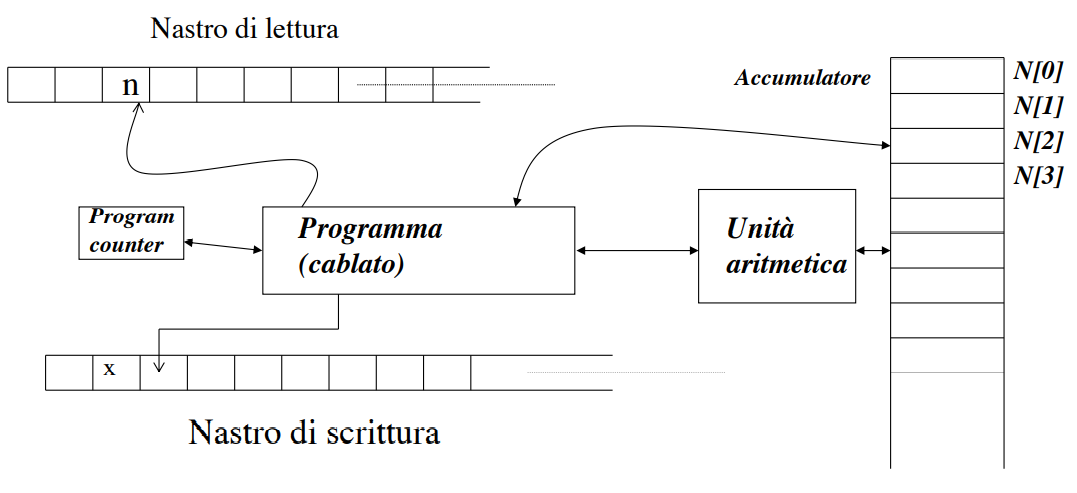
\includegraphics[width=\textwidth]{RAM.png}
  \end{figure}

  Sia i nastri che la memoria sono composti da un numero illimitato di celle, ma al contrario dei nastri di ingresso e uscita che si possono accedere in maniera sequenziale, la memoria è indirizzata e si può accedere a una sua cella attraverso un numero intero \(i>0\) che indica l'indirizzo di tale cella di memoria. La cella 0 della memoria è un registro speciale, detto accumulatore, che si utilizza per contenere il valore di uno dei due operandi delle operazioni aritmetiche binarie che la macchina può effettuare. Un generico programma eseguibile dalla macchina RAM è composto da istruzioni riportate nella tabella \ref{tabella istruzioni RAM}.

  \begin{table}[!h] 
    \caption{istruzioni macchina RAM}
    \vspace*{10pt}
    
    \centering
    \begin{tabular}{l l | l} \label{tabella istruzioni RAM}
      ISTRUZIONE & & SEMANTICA\\
      \hline
      LOAD= & \(x\) & M[0] \(\leftarrow x\)\\
      LOAD & \(x\)  & M[0] \(\leftarrow\) M[\(x\)]\\
      LOAD* & \(x\) & M[0] \(\leftarrow\) M[M[\(x\)]]\\
      STORE & \(x\) & M[\(x\)] \(\leftarrow\) M[0]\\
      STORE* & \(x\) & M[M[\(x\)]] \(\leftarrow\) M[0]\\
      ADD= & \(x\) & M[0] \(\leftarrow\) M[0] + \(x\)\\
      ADD  & \(x\)& M[0] \(\leftarrow\) M[0]+ M[\(x\)]\\
      ADD* & \(x\)& M[0] \(\leftarrow\) M[0] + M[M[\(x\)]]\\
      SUB= & \(x\)& M[0] \(\leftarrow\) M[0] - \(x\)\\
      SUB & \(x\)& M[0] \(\leftarrow\) M[0] - M[\(x\)]\\
      SUB* & \(x\)& M[0] \(\leftarrow\) M[0] - M[M[\(x\)]]\\
      MULT= & \(x\)& M[0] \(\leftarrow\) M[0] * \(x\)\\
      MULT & \(x\)& M[0] \(\leftarrow\) M[0] * M[\(x\)]\\
      MULT* & \(x\)& M[0] \(\leftarrow\) M[0] * M[M[0]]\\
      DIV= & \(x\)& M[0] \(\leftarrow\) M[0] \(\backslash\) \(x\) \\
      DIV & \(x\)& M[0] \(\leftarrow\) M[0] \(\backslash\) M[\(x\)]\\
      DIV* & \(x\)& M[0] \(\leftarrow\) M[0] \(\backslash\) M[M[\(x\)]]\\
      READ & \(x\)& M[x] \(\leftarrow\) input\\
      READ* & \(x\)& M[M[x]] \(\leftarrow\) input\\
      WRITE= & \(x\)& stampa \(x\)\\
      WRITE & \(x\)& stampa M[\(x\)]\\
      WRITE* & \(x\)& stampa M[M[\(x\)]]\\
      JUMP & \(label\)& PC \(\leftarrow\) \(label\) \\
      JGZ & \(label\)& PC \(\leftarrow\) \(label\) if M[0] \(>\) 0\\
      JLZ & \(label\)& PC \(\leftarrow\) \(label\) if M[0] \(<\) 0 \\
      JZ & \(label\)& PC \(\leftarrow\) \(label\) if M[0] = 0\\
      HALT & & terminazione\\
    \end{tabular}
  \end{table}

  Una volta introdotte tutte le istruzioni eseguibili dalla macchina RAM, è possibile ora studiarne la complessità temporale, come fatto per le TM a \(k\)-nastri. A differenza delle TM, nelle macchine RAM l'esecuzione delle diverse operazioni dipende dagli operandi necessari per eseguire tale operazione. Diventa quindi necessario analizzare tutte le istruzioni e definire il tempo richiesto per ciascuna di esse e la quantità di memoria allocata. Queste quantità possono essere calcolate secondo due criteri, ovvero tramite il criterio del costo costante e tramite il criterio del costo logaritmico. Il primo si basa sull'assunzione che l'esecuzione di ciascuna istruzione richieda un'unità di tempo e che ciascuna allocazione in memoria richieda un'unità di spazio (stessa assunzione fatta per le TM). 
  
  Si è appena affermato però che nella macchina RAM le istruzioni hanno diversa natura e manipolano dati di diversa dimensione: risulta, dunque, evidente che tale criterio è poco affine alla realtà. Per tener conto della differente velocità di esecuzione e della differente quantità di memoria allocata da ciascuna istruzione, si introduce il secondo criterio (del costo logaritmico), basato sulla supposizione che il tempo richiesto per eseguire un'istruzione sia proporzionale alla lunghezza degli operandi dell'istruzione considerata. Poichè gli operandi sono rappresentati in memoria in codice binario, un generico operando di valore \(v\) è rappresentato da \(\lfloor log_2(|v|+1)\rfloor\). 
  
  Dunque, è possibile definire la funzione \(l(i) = if\;i\neq 0\;then\;\lfloor log_2(|v|+1)\rfloor\;else\;1\) tramite cui calcolare la complessità temporale logaritmica di ciascuna istruzione precedentemente analizzata nella tabella \ref{tabella istruzioni RAM}. Alla stessa maniera, è possibile calcolare i costi relativi allo spazio, introducendo la variabile \(m\) definita come l'indirizzo più alto della cella di memoria a cui si fa accesso durante l'esecuzione del programma, e la variabile \(M_i\) che rappresenta il valore assoluto più grande immagazzinato in M[i] durante l'esecuzione. La complessità spaziale logaritmica si definisce quindi con la seguente formula:

  \(\displaystyle \sum_{i=0}^m{l(M_i)}\)\\
  Di seguito sono riportati i costi logaritmici delle istruzioni RAM:

  \begin{table}[!htb] \label{tabella costi logaritmici}
    \caption{costi logaritmici delle istruzioni macchina RAM}
    \vspace*{10pt}
    
    \centering
    \begin{tabular}{l l | l}
      ISTRUZIONE & & COSTO LOGARITMICO\\
      \hline
      LOAD= & \(x\) & \(l(x)\)\\
      LOAD & \(x\)  & \(l(x) + l(M[x])\) \\
      LOAD* & \(x\) & \(l(x) + l(M[x]) + l(M[M[x]])\)\\
      STORE & \(x\) & \(l(M[0]) + l(x)\)\\
      STORE* & \(x\) & \(l(M[0]) + l(x) + l(M[x])\)\\
      ADD= & \(x\) & \(l(M[0]) + l(x)\)\\
      ADD  & \(x\)& \(l(M[0]) + l(x) + l(M[x])\)\\
      ADD* & \(x\)& \(l(M[0]) + l(x) + l(M[x]) + l(M[M[x]])\)\\
      & & SUB, MULT, DIV definite come ADD.\\
      READ & \(x\)& \(l(input) + l(x)\)\\
      READ* & \(x\)& \(l(input) + l(x) + l(M[x])\)\\
      WRITE= & \(x\)& \(l(x)\)\\
      WRITE & \(x\)& \(l(x) + l(M[x])\)\\
      WRITE* & \(x\)& \(l(x) + l(M[x]) + l(M[M[x]])\)\\
      JUMP & \(label\)& 1 \\
      JGZ & \(label\)& \(l(M[0])\)\\
      JLZ & \(label\)& \(l(M[0])\) \\
      JZ & \(label\)& \(l(M[0])\)\\
      HALT & & 1\\
    \end{tabular}
  \end{table}
  
  Dunque, il criterio del costo costante si può applicare solo in situazioni in cui si prevede che ogni valore che comparirà durante l'esecuzione del programma occupi esattamente una cella di memoria, altrimenti si deve necessariamente applicare il criterio del costo logaritmico, che porta ad un calcolo più preciso della complessità.
  

  \section{Correlazione temporale fra TM e RAM}
  Una volta analizzato il comportamento della macchina RAM, è possibile studiarne la correlazione con le TM. Nello specifico, è possibile simulare una TM deterministica a \(k\) nastri attraverso una macchina RAM, nel seguente modo: innanzitutto, si considera la memoria della RAM come suddivisa in blocchi, tutti di dimensione \(k\), ad eccezione del blocco 0, che ha dimensione \(k+1\), in quanto memorizza lo stato della TM e le posizioni delle \(k\) testine. I successivi blocchi vengono impiegati per contenere i valori contenuti nelle successive posizioni di ciascuno dei \(k\) nastri di memoria della TM. Dunque, il valore rappresentato nella \(i\)-esima cella del \(j\)-esimo nastro della TM è contenuto nella locazione \(c+k\cdot j+i\) in cui \(c\) è una costante opportuna della memoria della macchina RAM. 
  Inoltre, per accedere al valore presente sotto la testina di lettura di un determinato nastro è prima necessario eseguire un accesso diretto al blocco 0, per poter trovare la posizione del nastro stesso. Poi, per eseguire la funzione di transizione \(\delta(q,i,s_1,...,s_k)\) e la funzione di uscita \(\eta(q,i,s_1,...,s_k)\), si richiedono un numero prefissato di accessi in memoria per ottenere \(q,i,s_1,...,s_n\), necessari per l'esecuzione di tali funzioni.

  Tutto ciò conduce al seguente teorema:

  \begin{theorem}
    Una TM multinastro con complessità temporale \(T_M\) può essere simulata da una macchina RAM con complessità temporale \(T_R = \Theta( T_M)\), secondo il criterio di costo uniforme, oppure \(T_R = \Theta( T_M \cdot log( T_M))\), secondo il criterio di costo logaritmico. 
  \end{theorem}

  Ovviamente è possibile anche simulare una macchina RAM tramite una macchina di Turing, ma tale costruzione è molto più complessa e richiede un'analisi approfondita. Si enuncia quindi solo il seguente teorema:

  \begin{theorem}
    Sia L il linguaggio riconosciuto da una macchina RAM di complessità temporale \({T}_R\) secondo il criterio del costo logaritmico. Se il programma RAM non utilizza le istruzioni \(MULT\) e \(DIV\), allora L può essere riconosciuto da un'opportuna TM multinastro, in un tempo \({T}_M=\Theta({T}_R^2)\). 
  \end{theorem}

  Si può quindi osservare come il legame tra \({T}_M\) e \({T}_R\) sia di tipo polinomiale, implicazione molto importante perchè suggerisce quale sia la classe di problemi trattabili nella pratica.
  \chapter{Algoritmi}
In questo capitolo si analizzano a fondo i principali algoritmi di ordinamento e i relativi tempi di esecuzione. Nello specifico, si utilizzerà come modello di riferimento la macchina RAM con un criterio di costo costante, come analizzato nei capitoli precedenti. Prima di proseguire nella trattazione è necessario dare una definizione generale di algoritmo:

\begin{definition}
  Un algoritmo è una procedura di calcolo ben definita che prende un certo valore, o un insieme di valori, in input e genera un valore, o un insieme di valori, in output. Dunque, un algoritmo è una serie di passi computazionali che trasformano l'input in output.
\end{definition}

Un algoritmo può anche essere visto come uno strumento per la risoluzione di un problema computazionale ben definito: sotto questo sguardo, un algoritmo si definisce corretto se, per ogni istanza di input, termina con l'output corretto. Se un algoritmo è corretto, allora risolve quel determinato problema computazionale. Esistono molti modi per poter specificare un determinato algoritmo: si può utilizzare la lingua italiana o inglese, ma anche un linguaggio di programmazione come C, C++, JAVA e Pascal, o ancora tramite uno pseudocodice.

\section{Pseudocodifica}
La pseudocodifica può avvenire in molti modi, ma nel seguito si utilizzerano le convenzioni qui riportate:
\begin{itemize}
  \item L'indentazione serve ad indicare la struttura a blocchi dello pesudocodice, in modo da comprendere quali istruzioni appartengono, per esempio, ad un ciclo for, a un ciclo while o ad un if-else statement. Non sono utilizzate le parentesi graffe o parole chiave come begin ed end in quanto appesantiscono la sintassi;
  \item I costrutti iterativi \code{while}, \code{for}, \code{repeat-until} e il costrutto condizionale \code{if-else} hanno interpretazioni simili a quelle dei comuni linguaggi di programmazione. Il contatore del ciclo mantiene il suo valore dopo la fine del ciclo, quindi il valore che ha provocato la terminazione del ciclo stesso. Inoltre, si utilizza la parola chiave \code{to} quando il ciclo \code{for} incrementa il valore del suo contatore ad ogni iterazione, mentre si utilizza la parola chiave \code{down to} nel caso la variabile venga decrementata;
  \item Le assegnazioni di un valore ad una certa variabile avviene con il simbolo \code{:=}, differente dall'operatore \code{=}, che invece indica l'eguaglianza di due valori all'interno di un costrutto \code{if};
  \item Per identificare un elemento appartenente ad un array, si utilizza la notazione con le parentesi quadre, al cui interno si indica l'indice dell'elemento a cui si vuole accedere: \code{array[i]}; Per indicare un intervallo di valori all'interno dell'array si utilizza la seguente sintassi: \code{array[i..j]}, con cui si indica la sottomatrice composta dagli elementi compresi fra \(i\) e \(j\); 
  \item I dati utilizzati sono tipicamente organizzati in oggetti, formati da attributi, a cui si accede tramite la notazione punto: \code{oggetto.proprietà}. Le variabili che rappresentano un determinato oggetto sono trattate come puntatori a tale oggetto. Un puntatore che non fa riferimento ad alcun oggetto è inizializzato con il valore \code{NIL};
  \item I parametri vengono passati ad una procedura per valore: la procedura chiamata riceve una sua copia dei parametri e, quindi, se a una di queste variabili è assegnato un nuovo valore, la modifica non è visibile dalla procedura chiamante. Nel caso venga passato come argomento un oggetto, viene copiato il puntatore a tale oggetto e quindi le modifiche sono visibili anche dalla procedura chiamante;
  \item L'istruzione \code{return} restituisce immediatamente il controllo al punto in cui la procedura chiamante ha effettuato la chiamata. Le istruzioni \code{return} possono anche ritornare un valore al chiamante;
  \item Gli operatori booleani \code{and} e \code{or} sono cortocircuitati. Ciò significa che nella valutazione dell'espressione \code{x and y}, si valuta prima se il valore di \code{x} sia falso, in quanto, se lo fosse, l'intera espressione sarebbe falsa e non avrebbe quindi alcun senso valutare il valore della variabile \code{y}. Al contrario, nella valutazione dell'espressione \code{x or y}, si verifica innanzitutto se il valore di \code{x} sia vero, in quanto, se lo fosse, l'intera espressione sarebbe vera e non avrebbe quindi alcun senso valutare il valore della variabile \code{y}.
\end{itemize}

Tramite queste regole è possibile definire un generico algoritmo.

\section{Insertion Sort}
Una classe di algoritmi molto studiati è quella riguardante l'ordinamento di un vettore, che consiste nella disposizione dei suoi elementi in ordine crescente.

\vspace{10pt}

Il primo algoritmo analizzato è l'\textbf{insertion sort}, che prende in input una sequenza di \(n\) numeri\\ \(<a_1, a_2, ...,a_n>\) e restituisce in output una permutazione \(<a_1', a_2',...,a_n'>\) tale che \(a_1'\le a_2' \le ... \le a_n'\).

Questo algoritmo ordina sul posto \footnote{L'algoritmo risistema gli elementi della sequenza all'interno dell'array avendo, in ogni istante, al più un numero finito di elementi memorizzati all'esterno dell'array: ciò permette di risparmiare memoria nel calcolatore.} gli elementi assumendo che la sequenza da ordinare sia inizialmente partizionata in una sottosequenza già ordinata, all'inizio composta da un unico elemento (il primo dell'array), e una sottosequenza ancora da ordinare. Ad ogni iterazione viene rimosso un elemento dalla sottosequenza non ordinata e inserita nella posizione corretta all'interno della sottosequenza già ordinata. 

In pseudocodice:

\lstinputlisting{../docs/insertion_sort.txt}

All'inizio di ogni iterazione del ciclo \code{for}, il cui indice è \(j\), la sottosequenza di elementi \code{A[1..j-1]} è la parte ordinata dell'array, mentre la sottosequenza \code{A[j+1..n]} è costituita da elementi ancora da ordinare.

\vspace{10pt}

Si analizza ora il tempo di esecuzione della procedura \code{insertion sort}: per ogni \(j=2,3,...,n\) in cui \(n\) = \code{A.length}, si indica con \(t_j\) il numero di volte che il test del ciclo \code{while} nella riga 5 viene eseguito per quel determinato valore di \(j\).



  \chapter{Strutture Dati}
Gli insiemi manipolati dagli algoritmi, a differenza di quelli matematici, possono essere modificati inserendo o rimuovendo elementi. Questi insiemi sono detti dinamici e giocano un ruolo importante in informatica, perchè modellano le strutture utilizzate per memorizzare in modo ordinato i dati.

In una tipica implementazione di un insieme dinamico, ogni elemento è rappresentato da un oggetto, i cui attributi possono essere esaminati e manipolati a piacimento dagli algoritmi. In molte strutture dati, l'oggetto dispone di una chiave identificativa (spesso univoca, ma non necessariamente) e ovviamente di dati satelliti che si vogliono memorizzare ordinatamente in memoria. Oltre a questi due attributi, l'oggetto può anche contenere altri dati specifici per una determinata struttura dati, in modo da rendere più semplice e veloce la loro manipolazione.

Le tipiche operazioni che si possono svolgere sulle strutture dati sono suddivise in due categorie: le query (interrogazioni), che hanno il solo scopo di estrapolare informazioni dall'insieme dinamico, e le operazioni di modifica, che hanno il compito di modificare l'insieme. Di seguito sono elencate le istruzioni più comuni:

\begin{itemize}
  \item \code{search(S, k)}: è un'operazione di query che, dato un insieme \(S\) e un valore chiave \(k\), restituisce \code{NIL} se tale elemento non appartiene all'insieme.
  \item \code{insert(S, x)}: è un'operazione di modifica che inserisce all'interno dell'insieme \(S\) l'elemento puntato da \(x\).
  \item \code{delete(S, x)}: è un'operazione di modifica che, dato un puntatore \(x\) ad un elemento dell'insieme \(S\), rimuove \(x\) da \(S\).
  \item \code{minimum(S)}: è un'operazione di query che ritorna l'elemento dell'insieme \(S\) con la chiave più piccola.
  \item \code{maximum(S)}: è un'operazione di query che ritorna l'elemento dell'insieme \(S\) con la chiave più grande.
  \item \code{successor(S, x)}: è un'operazione di query che, dato un elemento \(x\) la cui chiave appartiene ad un insieme totalmente ordinato \(S\), restituisce un puntatore all'elemento successivo più grande di \(S\) oppure \code{NIL} se \(x\) è il più grande degli elementi.
  \item \code{predecessor(S, x)}: è un'operazione di query che, dato un elemento \(x\) la cui chiave appartiene ad un insieme totalmente ordinato \(S\), restituisce un puntatore all'elemento precedente più piccolo di \(S\) oppure \code{NIL} se \(x\) è il più piccolo degli elementi.
\end{itemize}

\section{Stack}
Gli \textbf{stack} sono insiemi dinamici dove l'elemento da rimuovere tramite l'operazione \code{delete} è predeterminato. In questa struttura dati, l'elemento cancellato è quello inserito per ultimo, secondo la politica LIFO (Last In, First Out). Nello specifico, le operazioni di \code{insert} e \code{delete} prendono rispettivamente il nome di \code{push} e \code{pop} \footnote{Questa operazione non prende nessun argomento, in quanto l'elemento da eliminare è predeterminato}: la prima inserisce in cima alla pila l'elemento passato come argomento, mentre la seconda operazione elimina l'unico elemento accessibile dalla pila, ovvero la cima. 

Questa struttura dati può essere implementata tramite un array con un massimo di \(n\) elementi \code{S[1..n]}, che presenta lo specifico atrtibuto \code{S.top}, ovvero l'indice tramite cui accedere all'ultimo elemento inserito. L'array è dunque composto dagli elementi \code{S[1..S.top]}, dove \code{S[1]} rappresenta l'elemento in fondo alla pila, mentre \code{S[S.top]} rappresenta l'elemento in cima. Ovviamente, se \code{S.top} = 0, si dice che la pila è vuota, in quanto non contiene nessun elemento. In questo caso, se si tenta di estrarre un elemento dallo stack, si ottiene un errore di underflow dello stack, mentre se si cerca di inserire un elemento sulla pila piena (che conta quindi di \(n\) elementi), si ottiene un errore di overflow dello stack.

Le operazioni dello stack possono essere implementate molto semplicemente in pseudocodifica come segue:

\begin{lstlisting}
push(S, x):
  if S.top = S.length:
    error "overflow"
  else:
    S.top := S.top + 1
    S[S.top] := x
\end{lstlisting}

\begin{lstlisting}
pop(S):
  if iS.top = 0:
    error "underflow"
  else:
    S.top := S.top - 1
    return S[S.top + 1]
\end{lstlisting}

Si noti come, in questo caso, l'operazione di \code{pop} ritorna l'elemento appena eliminato dallo stack. Entrambe le procedure vengono eseguite in tempo costante \(\Theta(1)\).

\section{Queue}
Le \textbf{code} sono insiemi dinamici dove l'elemento da rimuovere tramite l'operazione \code{delete} è predeterminato. In questa struttura dati, l'elemento cancellato è quello inserito per primo, secondo la politica FIFO (First In First Out). Nello specifico, la coda presenta un inizio detto \code{head} e una fine detta \code{tail}, e le operazioni di \code{insert} e \code{delete} prendono rispettivamente il nome di \code{enqueue} e \code{dequeue} \footnote{Anche in questo caso, questa operazione non prende nessun argomento, in quanto l'elemento da eliminare è predeterminato}: la prima inserisce in fondo alla fila l'elemento passato come argomento, mentre la seconda operazione elimina il primo elemento della fila. 

Questa struttura dati può essere implementata tramite un array di \(n\) elementi \code{Q[1..n]}, che contiene un massimo di \(n-1\) elementi, per ragioni che verranno chiarite in seguito. L'attributo \code{Q.head} punta all'inizio della coda, mentre l'attributo \code{Q.tail} punta alla posizione in cui l'ultimo elemento che dovrà essere inserito prenderà posto (ovvero alla posiziove vuota successiva all'ultimo elemento della coda). Gli elementi della coda, quindi, occupano le posizioni \code{Q.head}, \code{Q.head + 1}, ..., \code{Q.tail - 1}. Alla fine dell'array la posizione 1 della queue segue immediatamete la posizione \(n\) secondo un ordine circolare. Se \code{Q.head = Q.tail} allora la coda è vuota. All'inizio le posizioni \code{Q.head} e \code{Q.tail} combaciano e sono entrambe inizializzate al valore 1.

Come per gli stack, se la coda è vuota, il tentativo di rimuovere un elemento provoca un errore di underflow, mentre se \code{Q.head = Q.tail + 1} la coda è piena e il tentativo di inserire un nuovo elemento provoca un errore di overflow. 

Le operazioni della queue possono essere implementate molto semplicemente in pseudocodifica come segue:

\begin{lstlisting}
enqueue(Q, x):
  Q[Q.tail] := x
  if Q.tail = Q.length:
    Q.tail := 1
  else:
    Q.tail := Q.tail + 1
\end{lstlisting}

\begin{lstlisting}
dequeue(Q, x):
  x := Q[Q.head]
  if Q.head = Q.length:
    Q.head := 1
  else:
    Q.head := Q.head + 1
  return x
\end{lstlisting}

Entrambe le procedure vengono eseguite in un tempo costante \(\Theta(1)\).

\section{Linked List}
Una \textbf{lista concatenata} è una struttura dati i cui oggetti sono disposti in ordine lineare, determinato da un puntatore in ogni oggetto. Una lista doppiamente concatenata è una lista in cui ogni oggetto presenta, oltre ad una chiave \code{key}, anche un puntatore all'elemento successivo \code{next} e un puntatore a quello precedente \code{prev}. Se \code{x.prev = NIL}, allora l'elemento \(x\) è il primo elemento della lista e si dice essere la testa (o head) della lista. Se, invece, \code{x.next = NIL}, allora \(x\) è l'ultimo elemento della lista e si dice essere la coda (o tail) della lista. Intuitivamente, l'attributo \code{L.head} punta alla testa della lista, che sarà vuota se \code{L.head = NIL}.

Questa struttura dati può presentare varie forme: può essere doppiamente concatenata o singolarmente concatenata, oppure può essere circolare o non. Una lista si dice singolarmente concatenata se i suoi oggetti non sono dotati di puntatore all'elemento precedente, mentre si dicono circolari se l'ultimo elemento possiede un puntatore alla testa della lista, che a sua volta possiede un puntatore alla coda se la lista è circolare. Una lista concatenata può anche essere ordinata o non: si dice ordinata quando la disposizione lineare degli elementi corrisponde con la disposizione crescente delle chiavi degli elementi e, in tal caso, la testa della lista conterrà l'elemento minimo, mentre la coda l'elemento massimo. 

Nel seguito si fa riferimento a liste non ordinate doppiamente concatenate per lo sviluppo degli algoritmi che le manipolano. 

\vspace{10pt}

La prima procedura che sia analizza è \code{listSearch(L, k)}, che trova il primo elemento con la chiave \(k\) nella lista \(L\), restituendo un puntatore a tale oggetto. Se nessun oggetto con chiave \(k\) è presente nella lista, allora viene restituito il valore \code{NIL}. In pseudocodifica:

\begin{lstlisting}
listSearch(L, k):
  x := L.head
  while x != NIL and x.key != key:
    x := x.next
  return x  
\end{lstlisting}

Si noti quindi che l'algoritmo \code{listSearch} cerca l'elemento di chiave \(k\) tramite una ricerca lineare sulla list \(L\) di \(n\) elementi. Dunque, l'algoritmo impiega un tempo \(\Theta(n)\) nel caso peggiore, in quanto potrebbe essere necessario scorrere l'intera lista.

\vspace{10pt}

La seconda procedura analizzata è \code{listInsert(L, x)} che inserisce l'elemento x di attributo key (già inizializzato) in testa alla lista. In pseudocodifica:

\begin{lstlisting}
listInsert(L, x):
  x.next := L.head
  if L.head != NIL:
    L.head.prev := x
  L.head := x
  x.prev := NIL 
\end{lstlisting}

Questa procedura impiega un tempo costante \(\Theta(1)\) per la sua esecuzione.

\vspace{10pt}

L'ultima procedura analizzata per le linked list è \code{listDelete(L, x)}, che rimuove l'elemento \(x\) dalla lista \(L\). Per poter eliminare tale elemento è prima necessario chiamare la funzione \code{listSearch} per ottenere il puntatore all'elemento desiderato. In pseudocodifica:

\begin{lstlisting}
listDelete(L, x):
  if x.prev != NIL:
    x.prev.next := x.next
  else:
    L.head := x.next
  if x.next != NIL:
    x.next.prev := x.prev
\end{lstlisting}

Anche questa procedura impiega un tempo di esecuzione \(\Theta(1)\).

\section{Hash Table}
\subsection{Indirizzamento diretto}
Prima di procedere con l'introduzione alle tavole di hash, è prima necessario introdurre il concetto di indirizzamento diretto, una tecnica molto efficiente nel caso in cui l'insieme da cui vengono acquisite le chiavi, detto insieme universo \(U = \{0,1,2...,m-1\}\), è un insieme ragionevolmente piccolo. Si suppone, inoltre, che due elementi distinti non possano avere chiavi coincidenti. Per rappresentare un tale insieme dinamico si utilizza un array, oppure una tavola ad indirizzamento diretto, indicata con \(T[0..m-1]\), dove ogni cella \(k\) di tale tabella punta all'elemento dell'insieme di chiave \(k\). Se la \(k\)-esima cella non contiene nessun elemento, viene inizializzata con il valore \code{NIL}.

Le operazioni di dizionario sono semplici da implementare in pseudocodifica e impiegano tutte un tempo costante \(O(1)\) (nel caso peggiore):

\begin{lstlisting}
directAddressSearch(T, k):
  return T[k]
\end{lstlisting}

\begin{lstlisting}
directAddressInsert(T, x):
  T[x.key] := x 
\end{lstlisting}

\begin{lstlisting}
directAddressDelete(T, x):
  T[x.key] := NIL
\end{lstlisting}

In alcune implementazioni è possibile memorizzare l'elemento di chaive \(k\) direttamente all'interno della tabella, anzichè in un oggetto esterno, risparmiando spazio in memoria. 

\subsection{Introduzione alle Tavole di Hash}

La difficoltà nell'implementazione di una tale struttura dati è evidente: l'insieme universo \(U\), nella maggior parte dei casi, è troppo grande per essere memorizzato in una tavola \(T\) di dimensione \(|U|\). Inoltre, l'insieme \(K\) delle chiavi effettivamente memorizzate è molto più piccolo dell'inisieme \(U\) delle chiavi disponibili e, dunque, la maggior parte dello spazio allocato per la tavola \(T\) non verrebbe mai utilizzato. A questo proposito si introduce una nuova struttura dati, detta \textbf{tavola di hash}, che utilizza una memoria proporzionale al numero delle chiavi effettivamente memorizzate nel dizionario, riducendo lo spreco di memoria. 

Quando l'insieme \(K\) delle chiavi memorizzate in un dizionario è molto più piccolo dell'universo \(U\) di tutte le chiavi possibili, utilizzando una tavola di hash si può ridurre lo spazio richiesto fino a \(\Theta(|K|)\), rdiucendo però l'efficienza temporale a \(O(1)\) nel caso medio (anzichè pessimo). Nella tabella di hash, l'elemento di chiave \(k\) non viene memorizzato direttamente nella cella \(k\), ma viene utilizzata una cosiddetta funzione di hash \(h(k)\) che calcola l'indice \(k\) della cella. La funzione di hash \(h(k)\) associa ad ogni chiave dell'universo \(U\) una specifica chiave della tavola di hash \(T[0..m-1]\). Formalmente:

\(h(k):U\to \{0,1,..., m-1\},\;\;\; m<<|U|\)

Si dice che \(h(k)\) è il valore hash della chiave \(k\).

\subsection{Hashing Concatenato}

Il problema principale con la tecnica di indirizzamento appena analizzata è che, riducendo l'intervallo degli indici da \(|U|\) ad \(m<<|U|\), è molto probabile che due chiavi vengano mappate nella stessa cella: in tal caso si dice che avviene una collisione. Per evitare un evento simile è possibile, in prima analisi, implementare una funzione di hash totalmente deterministica il più randomica possibile, in modo da minimizzare le collisioni. Si dimostra però che un evento di collisione è impossibile da evitare in quanto \(|U| > m\) e quindi, dopo l'\(m\)-esima chiamata alla funzione di hash, avverà sicuramente una collisione. 

Si rende necessario, dunque, implementare un meccanismo che gestisca tali eventi. Nello specifico, la tecnica più utilizzata è il concatenamento (o chaining), tramite cui, tutti gli elementi associati ad una stessa cella \(k\) sono posti in una lista concatenata. La cella \(k\), in questo caso, punta al nodo di testa della lista che contiene gli elementi mappati in tale cella, oppure ha valore \code{NIL}, nel caso in cui la cella non contenga nessun elemento. 

Le operazioni di dizionario su una tavola di hash \(T\) sono facili da implementare in pseudocodifica nel caso di gestione delle collisioni tramite concatenamento:

\begin{lstlisting}
chainedHashInsert(T, x):
  listInsert(T[h(x.key)], x)
\end{lstlisting}

\begin{lstlisting}
chainedHashSearch(T, x):
  listSearch(T[h(x.key)], x)
\end{lstlisting}

\begin{lstlisting}
chainedHashDelete(T, x):
  listDelete(T[h(x.key)])
\end{lstlisting}

In cui le procedure \code{listInsert}, \code{listSearch} e \code{listDelete}, sono le stesse analizzate nella sezione delle liste concatenate e hanno il compito, rispettivamente, di inserire in testa alla lista un nodo, cercare un nodo nella lista ed eliminare un nodo dalla lista. 

Si passa ora all'analisi del tempo di esecuzione di tali procedure: nel caso peggiore, l'inserimento in lista di un nodo è \(O(1)\), la ricerca avviene in tempo proporzionale alla lunghezza della lista, quindi \(O(n)\), mentre l'eliminazione di un nodo dalla lista avviene, sempre nel caso peggiore, in tempo \(O(1)\) se la lista è doppiamente concatenata. 

Si noti che la funzione \code{chainedHashDelete} prende come input un elemento \(x\), non la sua chiave \(k\), quindi non occorre cercare prima l'elemento \(x\). Se la tavola di hash supporta la cancellazione, allora le sue liste dovrebbero essere doppiamente concatenate in modo che la cancellazione di un elemento sia più rapida. Se le liste fossero singolarmente concatenate, per cancellare l'elemento \(x\), si dovrebbe prima trovare \(x\) nella lista \(T[h(x.key)]\) in modo da poter aggiornare l'attributo \code{next} dell'elemento precedente in lista, assegnandogli il valore \code{NIL}.

\subsection{Analisi della Funzione di Hash}
Data una tavola di hash \(T\), che conta \(m\) celle in cui sono memorizzati \(n\) elementi, si definisce il fattore di carico \(\alpha\) della tavola \(T\) come il rapporto \(n/m\), ossia il numero medio di elementi memorizzati in una lista. Il caso peggiore nell'hashing si verifica quando tutte le \(n\) chiavi sono associate alla stessa cella, creando una lista di lunghezza \(n\). Il tempo di esecuzione della ricerca diventa quindi \(\Theta(n)\) a cui si aggiunge il tempo di esecuzione della funzione di hashing. Ovviamente, un caso del genere è molto improbabile nel caso in cui la funzione di hash sia ben progettata. Per il momento si suppone che ogni elemento ha uguale probabilità di essere mappato in una qualsiasi delle \(m\) celle, indipendentemente dalle celle in cui sono stati mappati gli altri elementi. Tale ipotesi viene definita hashing uniforme semplice. Per ogni \(j=0,1,..., m-1\), si indica con \(n_j\) la lunghezza della lista \(T[j]\), ottenendo quindi il numero di elementi totali memorizzati in tabella è \(n=n_0+n_1+...+n_{m-1}\). Il valore atteso di ogni \(n_j\) sarà \(E[n_j] = \alpha = n/m\), quindi il tempo medio per la ricerca di un elemento di chiave \(k\) non presente nella lista (caso pessimo) è \(\Theta(1+\alpha)\), che si dimostra essere anche il tempo di ricerca dello stesso elemento, questa volta presente tabella. Nella pratica, se il numero di celle nella tavola di hash è almeno proporzionale al numero di elementi della tavola, si ottiene che \(n=O(m)\) e quindi \(\alpha = n/m = O(m)/m = O(1)\). Pertanto, la ricerca di un elemento della tavola richiede un tempo costante.Ogni operazione di dizionario può essere svolta, in media, in un tempo \(O(1)\).

\subsection{Funzione di Hash}
Per progettare una buona tabella di hash è necessario implementare una funzione di hash che sia altamente efficiente. A questo proposito si introducono tre possibili schemi di implementazione: hashing per divisione (uristico), hashing per moltiplicazione (euristico) e hashing universale (aleatorio, non analizzato in questa sezione). In generale, una buona funzione di hashing deve soddisfare approssimativamente la condizione di hashing uniforme semplice: ogni chiave deve avere la stessa probabilità di essere mappata in una qualsiasi cella della tabella. Di solito non è possibile verificare questa condizione, in quanto non è nota la distribuzione delle probabilità secondo cui vengono estratte le chiavi. Quindi, nella pratica, spesso si utilizzano delle tecniche euristiche per la realizzazione di tali funzioni.

La maggior parte delle funzioni di hashing suppone che l'universo delle chiavi sia l'insieme dei numeri naturali \(\mathbb{N}\) e quindi, se nella struttura dati progettata, la chiave non è un numero naturale ma, ad esempio, una stringa, è necessario studiare un metodo di conversione: nei calcolatori questo metodo è tipicamente già implementato, in quanto ogni informazione analogica viene convertita in una stringa binaria di bit (appartenente ad \(\mathbb{N}\)). Nello studio dei tre metodi di hashing si suppone che le chiavi siano numeri naturali.

\vspace{10pt}

\textbf{Metodo della Divisione}. Quando si applica il metodo della divisione per creare una funzione di hash, una chiave \(k\) viene associata a una delle \(m\) celle prendeno il resto della divisione fra \(k\) ed \(m\). Formalmente, la funzione di hash è così definita:

\(h(k)=k\; mod\; m\)

\noindent Il vantaggio principale di questo metodo è che si può implementare molto rapidamente e richiede un tempo di esecuzione costante. 

Quando si utilizza il metodo della divisione, si cerca di evitare alcuni valori di \(m\). Nello specifico si evitano le potenze di 2, in quanto se \(m=2^p\), allora \(h(k)\) rappresenta proprio i \(p\) bit meno significativi di \(k\): infatti, sarebbe più corretto far dipendere la funzione di hash da tutti i bit della chiave. Inoltre, si evita di scegliere \(m+2^p-1\) quando \(k\) è una stringa di caratteri interpretata in base \(2^p\), in quanto la permutazione dei caratteri di \(k\) non cambia il suo valore di hash. Una buona scelta di \(m\), invece, potrebbe essere un numero primo non troppo vicino a una potenza esatta di 2.

\vspace{10pt}

\textbf{Metodo della Moltiplicazione}. Il metodo della moltiplicazione per la creazione di funzioni di hash consiste in due passi. Nel primo passaggio si moltiplica la chiave \(k\) per una costante \(A\), tale che \(0<A<1\), per poi estrarre la parte frazionaria del numero appena ottenuto. Nel secondo passaggio si moltiplica questo valore per \(m\) e si prende la parte intera inferiore del risultato. Formalmente, la funzione di hash è così definita:

\(h(k) = \lfloor m\,(k\cdot A\;mod\;1)\rfloor\)

\noindent dove \(k\cdot A \; mod \;1 \) rappresenta la parte frazionaria di \(kA\), ovvero \(kA-\lfloor kA\rfloor\). 

Il vantaggio principale di questo metodo è che il valore di \(m\) non è critico. Tipicamente si sceglie un valore di \(m\) tale per cui sia una potenza di 2, in modo da rendere più semplice implementare tale funzione in un calcolatore reale. Si upponga, infatti, che la dimensione di una parola nel calcolatore sia \(w\) bit e che il numero \(k\) sia contenuto in una sola parola. Si scelga poi un valore di \(A\) che sia una frazione nella forma \(s/2^w\), con \(s\) intero nell'intervallo \(0<s<2^w\). A questo punto, si moltiplica \(k\) per \(s=A\cdot 2^w\): il risultato sarà un numero di \(2w\) bit \(r_1 2^w+r_0\), in cui \(r_1\) rappresenta la parte più significativa del prodotto ed \(r_0\) la parte meno significativa. Il valore hash desiderato di \(p\) bit è formato dai \(p\) bit più significativi di \(r_0\). Sebbene queste operazioni funzionino con qualsiasi valore della costante \(A\), la scelta spesso adoperata è \(A \approx (\sqrt{5}-1)/2 \approx 0.6180339887...\)

\subsection{Indirizzamento Aperto}
UN altro metodo per evitare le collisioni è tramite l'indirizzamento aperto, in cui tutti gli elementi sono memorizzati nella tavola hash, ovvero ogni cella contiene un elemento dell'insieme dinamico o la costante \code{NIL} se non contiene nessun elemento. Quando si cerca un elemento, si esamina sistematicamente la tabella fino a quando non si trova l'elemento desiderato, oppure finchè non ci sono più elementi da controllare (l'elemento non è nell'array). Nell'indirizzamento aperto, a differenza degli altri metodi, la tavola hash può riempirsi fino a quando non può più fisicamente contenere altri elementi. Una conseguenza di questo design è che il fattore di carico \(\alpha\) non supera mai il valore 1. Il vantaggio di questo metodo sta nel fatto che elimina completamente l'utilizzo dei puntatori, in quanto calcola la sequenza delle celle da esaminare, e libera quindi una notevole quantità di memoria, utilizzata per incrementare la capacità della tabella, riducendo il rischio di collisioni. 

Per effettuare un insierimento mediante il metodo dell'indirizzamento aperto, si esamina in successione le posizioni della tavola hash fino a che non si trova una cella libera in cui inserire la chiave. L'efficienza di questo metodo consiste nel calcolare una nuova sequenza di accesso alla tabella in base alla chiave dell'oggetto da inserire, anzichè seguire sempre lo stesso cammino di accessi, che impiegherebbe un tempo di esecuzione \(\Theta(n)\). Per determinare quali celle esaminare durante la fase di ispezione, si estende la funzione di hash in modo da includere l'ordine di ispezione (a partire da 0), come secondo input. Formalmente, la funzione di hash modificata è definita come segue:

\(h(k,i):U\times \{0,1,...,m-1\} \to \{0,1,...,m-1\}\)

\noindent Si richiede, inoltre, che per ogni chiave \(k\) la sequenza di ispezione \(<h(k,0), h(k,1),..., h(k,m-1)>\) sia una permutazione della sequenza \(<0,1,...,m-1>\), in modo tale che ogni cella della tavola possa essere considerata come possibile cella in cui inserire una nuova chiave. In pseudocodifica:

\begin{lstlisting}
hashInsert(T, k):
  i := 0
  repeat
    j := h(k, i)
    if T[j] = NIL or T[j] = DELETED:
      T[j] := k
      return j
    else:
      i := i + 1
  until i = m
  error "hash table overflow"
\end{lstlisting}

Questa procedura prende in input una tavola di hash \(T\) e una chiave \(k\) da inserire in tabella, e ritorna l'indice della cella in cui è stato inserito l'elemento, oppure \code{error} di overflow se non è presente nessuna cella libera. Si noti nella condizione in riga 5, che viene verificato se la cella \(T[k]\) contiene il valore \code{DELETED}: questo valore speciale verrà ripreso e analizzato più avanti, con la procedura di eliminazione delle chiavi dalla tabella.

\vspace{10pt}

Per la ricerca di una determinata chiave \(k\) esamina la stessa sequenza di celle che ha esaminato l'algoritmo di inserimento quando ha inserito l'elemento di chiave \(k\). Dunque, la procedura di ricerca potrebbe terminare la propria esecuzione senza successo quando trova una cella vuota, in quanto la chiave \(k\) sarebbe stata inserita in quella posizione (si presuppone che le chiavi non possano essere eliminate dalla tavola). In pseudocodifica:

\begin{lstlisting}
hashSearch(T, k):
  i := 0
  repeat
    j := h(k, i)
    if T[j] = k:
      return j
    i := i + 1
  until T[j] = NIL or i = m
  return NIL
\end{lstlisting}

Questa procedura, come la precedente, prende in input una tavola di hash \(T\) e una chiave \(k\) da ricercare in tabella, e ritorna l'indice della cella in cui è stato trovato l'elemento, oppure \code{NIL} se non è presente nessuna cella che contiene l'elemento oppure se nella sequenza di ricerca si trova una cella libera (per le ragioni precedentemente analizzate).

\vspace{10pt}

La procedura di cancellazione di una chiave dalla tavola di hash ad indirizzamento aperto è un'operazione molto complessa, in quanto non è possibile semplicemente cancellare il contenuto della cella \(i\), assegnandone il valore \code{NIL}, in quanto sarebbe impossibile ricercare qualsiasi elemento in tabella per come è stata definita la procedura di ricerca. Dunque, si rende necessario marcare la cella il cui contenuto è stato eliminato con il valore speciale \code{DELETED}, anzichè \code{NIL}. È per questo motivo che in riga 5 della procedura di inserimento viene anche verificato se la cella ispezionata contanga il valore \code{DELETED}. Si noti inoltre che, utilizzando questa nuova notazione, il tempo di esecuzione della procedura di ricerca non dipende più dal fattore di carico \(\alpha\). Per questo motivo, nella pratica si preferisce spesso utilizzare il metodo della concatenazione quando è necessario che la tabella di hash supporti l'operazione di cancellazione delle chiavi. 

\vspace{10pt}

Nell'analisi delle tabelle hash con indirizzamento aperto si ipotizza hashing uniforme: si suppone, infatti, che ogni chiave abbia la stessa probabilità di avere come sequenza di ispezione una delle \(m!\) permutazioni di \(<0,1,...,m-1>\). L'hashing uniforme estende il concetto di hashing uniforme semplice, impiegato più volte precedentemente, al caso in cui la funzione di hash produce, non un singolo numero, ma un'intera sequenza di ispezione. Nella pratica non è possibile ottenere una funzione di hash uniforme, ma si utilizzano delle approssimazioni accettabili. Si esaminano nel seguito tre tecniche utilizzate per calcolare le sequenze di ispezione richieste nell'indirizzamento aperto: ispezione lineare, ispezione quadratica e doppio hashing. Tali tecniche grantiscono che la sequenza \(<h(k,0), h(k,1),..., h(k,m-1)>\) sia una permutazione di \(<0,1,...,m-1>\) per ogni chiave \(k\), ma nessuna di loro può garantire l'ipotesi di hashing uniforme, in quanto nessuna di esse è in grado di generare più di \(m^2\) sequenze di ispezioni differenti (invece delle \(m!\) sequenze richieste). 

\vspace{10pt}

\textbf{Ispezione Lineare}. Data una funzione di hash ordinaria \(h':U\to \{0,1,...,m-1\}\), detta funzione di hash ausiliaria, il metodo di ispezione lineare utilizza la funzione di hash

\(h(k,i)=(h'(k)+i)\;mod\;m\)

\noindent per \(i=0,1,...,m-1\). Data la chiave \(k\), la prima cella esaminata è \(T[h'(k)]\), che è la cella data dalla funzione di hash ausiliaria, la seconda cella è \(T[h'(k)+1]\) e così via fino alla cella \(T[m-1]\). Poi, l'ispezione riprende dalle celle \(T[0], T[1],...,T[h'(k)-1]\). Poichè la prima cella ispezionata determina l'intera sequenza di ispezioni, ci sono soltanto \(m\) sequenze di ispezione distinte. Questa tecnica è facile da implementare ma presenta un problema noto come addensamento primario: si formano lunghe file di celle occupate che aumentano il tempo medio di ricerca. Tale fenomeno si presenta perchè una cella vuota preceduta da \(i\) celle piene ha probabilità \((i+1)/m\) di essere la prossima ad essere occupata e le lunghe file di celle occupate tendono, dunque, a diventare sempre più lunghe.

\vspace{10pt}

\textbf{Ispezione Quadratica}. Data la funzione di hash ausiliaria \(h':U\to \{0,1,...,m-1\}\), il metodo di ispezione qudratica utilizza la funzione di hash

\(h(k,i)=(h'(k)+c_1i+c_2i^2)\;mod\;m\)

\noindent per \(i=0,1,...,m-1\), con \(c_1, c_2 \neq 0 \) costanti ausiliarie. Data la chiave \(k\), la prima cella esaminata è \(T[h'(k)]\), mentre le successive posizioni esaminate sono distanti dalle precedenti di quantità che dipendono in modo quadratico dal numero d'ordine di ispezione \(i\). Questa tecnica funziona meglio della precedente, ma i valori \(c_1, c_2\) ed \(m\) non possono essere scelti in maniera arbitraria, ma devono essere tali per cui si possa percorrere l'intera tabella. Inolte, se due chiavi hanno la stessa posizione iniziale di ispezione, allora le due sequenze di ispezione saranno identiche portando al cosiddetto addensamento secondario.

\vspace{10pt}

\textbf{Doppio Hashing}. Date la funzioni di hash ausiliarie \(h_1\) ed \(h_2\), il metodo di ispezione lineare utilizza la funzione di hash

\(h(k,1) = (h_1(k)+ih_2(k))\;mod\;m\)

\noindent per \(i=0,1,...,m-1\). Il doppio hashing è il metodo migliore disponibile per l'indirizzamento aperto, in quanto le permutazioni prodotte hanno molte caratteristiche comuni con le permutazioni casuali. Data la chiave \(k\), la prima cella esaminata è \(T[h_1(k)]\), mentre le successive posizioni sono distanziate dalle precedenti di quantità \(h_2(k)\;mod\;m\). Differentemente dai precedenti, il metodo del doppio hashing produce sequenze che dipendono in due modi dalla chiave \(k\), in quanto possono variare sia la posizione iniziale della sequenza di ispezione, sia la distanza fra due posizioni successive. 

Inoltre, il valore \(h_2(k)\) deve essere relativamente primo con la dimensione \(m\) della tavola hash perchè venga ispezionata l'intera tabella. Un modo pratico per garantire tale condizione è scegliere \(m\) potenza di due e definire \(h_2\) in modo che produca sempre un numero dispari. Un altro modo è scegliere \(m\) primo e definire \(h_2\) in modo che generi sempre un numero intero positivo minore di \(m\). In questo contesto, il doppio hashing è migliore delle precedenti tecniche in quanto utilizza \(\Theta(m^2)\) sequenze di ispezione, anzichè \(\Theta(m)\), perchè ogni possibile coppia di \(h_1, h_2\) produce una distinta sequenza di ispezione.





% \section{Alberi Binari}
% \section{Alberi RB}
% \section{Grafi}

  \chapter{Grammatiche}
  Come visto in precedenza, spesso gli automi vengono utilizzati come modelli per il riconoscimento di linguaggi. Gli automi sono quindi uno strumento formale per la descrizione e la definizione di un determinato linguaggio, costituito dall'insieme delle stringhe accettate dall'automa stesso.

  Un altro formalismo utilizzato per la definizione di linguaggio sono le cosiddette grammatiche formali, che definiscono un linguaggio fornendo il procedimento mediante cui si ottengono le stringhe appartenenti al linguaggio stesso. 
  
  \section{Introduzione}

  Una grammatica formale è un insieme di regole per costruire stringhe appartenenti ad un determinato linguaggio, attraverso il meccanismo di riscrittura, che consiste in un insieme di tecniche che determinano come sostituire le parti di una formula con parti più semplificate. In generale, un meccanismo di riscrittura consiste in un insieme di regole linguistiche, di cui una descrive l'oggetto principale come una sequenza di componenti. Ogni componente si può raffinare da elementi via via sempre più dettagliati, fino ad ottenere una sequenza di componenti elementari.

  Una grammatica non è altro che un meccanismo linguistico, composto dall'oggetto principale, detto anche simbolo iniziale, da un insieme di componenti, a loro volta da sostituire durante il processo di derivazione, detti anche simboli non terminaliun insieme di elementi di base, detti anche simboli elementari, e da un insieme di regole di raffinamento o sostituzioni, chiamate produzioni.

  \begin{definition} \label{definizione grammatica}
    Una grammatica G è una tupla di 4 elementi \(G = <V_T, V_N, P, S>\), dove:
    \begin{itemize}
      \item \(V_T\) è un insieme di simboli terminali (solitamente indicati con lettere minuscole), detto anche alfabeto terminale;
      \item \(V_N\) è un insieme di simboli non terminali (solitamente indicati con lettere maiuscole), tali che \(V_T \cap V_N = \emptyset\), detto anche alfabeto non terminale; V indica \(V_T\cup V_N\);
      \item P è un insieme finito di \(V_N^+\times V^*\), detto anche insieme delle produzioni di G. Un elemento \(p=<\alpha, \beta> \in P\) si indica con \(\alpha\to\beta\), in cui \(\alpha\) è la parte sinistra di p, mentre \(\beta\) è la parte destra di p;
      \item S è un elemento particolare di \(V_N\), detto assioma o simbolo iniziale. 
    \end{itemize}
  \end{definition}

  Quindi, un elemento che deve essere ancora raffinato è un simbolo non terminale, un elemento di base è un simbolo terminale, le componenti di un oggetto possono essere sia simboli terminali che non terminali, mentre una produzione corrisponde ad una regola di raffinamento.

  \begin{definition}
    Data una grammatica G, si definisce su \(V^*\) la relazione binaria di derivazione immediata, indicata con il simbolo \(\Rightarrow\) da \(\alpha\) a \(\beta\). Tale relazione sussiste se e solo se \(\alpha=\alpha_1\gamma\alpha_2, \beta=\alpha_1\delta\alpha_2\), con \(\alpha_1, \alpha_2, \delta \in V^*, \gamma \in V_N^+, \gamma\to\delta\in P\).
  \end{definition}

  Data la definizione di derivazione immediata, si può anche definire la chiusura riflessiva e transitiva, indicata con il simbolo \(\Rightarrow^*\), che opera su una serie di stringhe (di simboli elementari o non elementari), anzichè che su una sola stringa.

  Date le precedenti definizioni, si può ora definire il linguaggio generato da una grammatica, tramite la seguente definizione:
  \begin{definition}
    Data una grammatica G, il linguaggio L(G) generato da G è definito come:

    \(L(G)=\{x\;|\;S\Rightarrow^*x, x\in V_T^*\}\)
  \end{definition}

  Quindi il linguaggio generato da una grammatica è costituito da tutte e sole le stringhe di simboli terminali, derivati a partire dall'assioma \(S\), applicando un numero qualsiasi di sostituzioni.

  \section{Classificazione}
  Una volta definite cosa siano le grammatiche, è possibile classificarle in base alle loro proprietà e in base alla forma ammessa per le produzioni. Tale classificazione viene anche detta Gerarchia di Chomsky, tramite cui si dividono le grammatiche in quattro categorie:
  \begin{itemize}
    \item Grammatiche di tipo 0 (non ristrette): sono grammatiche definite come nella \ref{definizione grammatica}, ovvero grammatiche che non possiedono nessuna restrizione nel tipo di produzione;
    \item Grammatiche di tipo 1 (sensibili al contesto): sono grammatiche a cui si introduce il vincolo per cui le produzioni possono essere solo nella forma \(\alpha A\beta\to\alpha\gamma\beta\), dove \(\alpha, \beta, \gamma\in V\) e \(A\in V_N\), con \(\gamma\neq\varepsilon\); inoltre, la derivazione \(S\to\varepsilon\) è consentita solo se \(S\) non appare a destra in nessuna regola di derivazione;
    \item Grammatiche di tipo 2 (non contestuali): sono grammatiche a cui si introduce il vincolo per cui ad ogni produzione \(\alpha\to\beta \in P\) si verifica che \(\;|\;\alpha\;|\; =1\) (quindi \(\alpha \in V_N\)) e \(\beta\in V^*\);
    \item Grammatiche di tipo 3 (regolari): sono grammatiche a cui si introduce il vincolo per cui ad ogni produzione \(\alpha\to\beta \in P\) si verifica che \(\;|\;\alpha\;|\; = 1\) (quindi \(\alpha \in V_N\)) e che \(\beta\) sia in una sola delle seguenti forme: \(aB\), \(Ba\), \(a\) oppure \(\varepsilon\), con \(a\in V_T\) e \(B\in V_N\); inoltre, la derivazione \(S\to\varepsilon\) è consentita solo se \(S\) non appare a destra in nessuna regola di derivazione;
  \end{itemize} 

  \begin{figure}[!h]
    \begin{center}    
      \begin{tikzpicture}
        \foreach \X [count=\Y starting from 0.75] 
        in {tipo 3, tipo 2, tipo 1, tipo 0} {
          \draw (-\Y,-\Y/2) circle ({1.5*\Y} and \Y);
          \node at (1-2*\Y,-1.1*\Y) {\X}; 
        }
      \end{tikzpicture}
    \end{center}
    \caption{Gerarchia di Chomsky}    
  \end{figure}

  \section{Grammatiche e Automi}
  Studiando le grammatiche e i linguaggi da esse generate, si può osservare una certa corrispondenza con gli automi analizzati nei capitoli precedenti. Si introducono qui alcuni teoremi che mettono in luce la correlazione esistente fra automi e grammatiche.

  \begin{theorem}
    Dato un FSA A, è possibile costruire una grammatica regolare (di tipo 3) G ad esso equivalente, ossia in grado di riconoscere lo stesso linguaggio riconosciuto da A, e viceversa. Dunque, le grammatiche regolari e gli automi a stati finiti sono modelli differenti per descrivere la stessa classe di linguaggi. 
  \end{theorem}
  Dato un FSA \(A=<I, \delta, q_0, F>\), si può costruire una grammatica \(G=<V_N,V_T, P, S>\) regolare, tale che:
  \begin{itemize}
    \item \(V_N=Q\);
    \item \(V_T=I\);
    \item \(S=q_0\);
    \item \(\forall B\to bC\iff C\in\delta(B,b)\);
    \item \(\forall B\to\varepsilon, B\in F\)
  \end{itemize}
  Data una grammatica \(G=<V_N, V_T, P, S>\) regolare, si può costruire un FSA \(A=<I, \delta, q_0, F>\), tale che:
  \begin{itemize}
    \item \(Q=V_N\cup\{q_F\}\);
    \item \(I=V_T\);
    \item \(q_0=S\);
    \item \(F=\{q_F\}\)
    \item \(\forall A\to bC, C\in \delta(A,B)\);
    \item \(\forall A\to b, q_F\in\delta(A,b)\)
  \end{itemize}

  In generale, l'automa a stati finiti \(A\), ottenuto a partire dalla grammatica regolare \(G\), è non deterministico.

  \begin{theorem}
    Dato un NPDA A è possibile costruire una grammatica G non contestuale (di tipo 2) ad esso equivalente, ossia in grado di riconoscere lo stesso linguaggio riconosciuto da A, e viceversa. Dunque, le grammatiche non contestuali e gli automi a pila non deterministici sono modelli differenti per descrivere la stessa classe di linguaggi.
  \end{theorem}

  \begin{theorem}
    Data una TM M utilizzata come accettatore di linguaggi è possibile costruire una grammatica generale G (di tipo 0) ad essa equivalente, ossia in grado di riconoscere lo stesso linguaggio riconosciuto da M, e viceversa.Dunque, le grammatiche non ristrette e le macchine di Turing sono modelli differenti per descrivere la stessa classe di linguaggi.
  \end{theorem}

  \section{Espressioni Regolari}
  Un'espressione regolare è un'espressione utilizzabile per denotare un linguaggio attraverso la struttura delle stringhe che lo compongono.

  \begin{definition}
    Dato un alfabeto di simboli terminali denotato con \(V_T\), si definiscono su di esso le espressioni regolari e i corrispondenti linguaggi denotati:
    \begin{itemize}
      \item \(\emptyset\) è un'espressione regolare che denota il linguaggio vuoto;
      \item \(\forall a\in V_T, a\) è un'espressione regolare che denota il linguaggio formato solo dal simbolo \(a\);
      \item Se \(R_1\) ed \(R_2\) sono espressioni regolari, anche la loro unione, indicata con \(R_1+R_2\) o \(R_1\;|\;R_2\), è un'espressione regolare;
      \item Se \(R_1\) ed \(R_2\) sono espressioni regolari, anche la loro concatenazione, indicata con \(R_1\cdot R_2\), è un'espressione regolare;
      \item Se R è un'espressione regolare, anche la stella di Kleene di R, indicata con \(R^*\), è un'espressione regolare.
    \end{itemize}
  \end{definition}

  Nessun'altra stringa è un'espressione regolare.

  Gli operatori \(\;|\;, \cdot, ^*\) definiti per le espressioni regolari, hanno un implicito ordine di applicazione, se non indicato diversamente dall'uso delle parentesi. In particolare, * ha la precedenza rispetto a \(\cdot\), che ha a sua volta la precedenza su \(\;|\;\).
  
  Inoltre, vale anche il seguente teorema:
  \begin{theorem}
    La classe dei linguaggi denotati dalle espressioni regolari coincide con la classe dei linguaggi regolari. 
  \end{theorem}

  \section{Pattern}

  \begin{definition}
    Un sistema di pattern è una tripla \(<A, V, p>,\) dove:
    \begin{itemize}
      \item \(A\) è un alfabeto;
      \item \(V\) è un insieme di variabili tale che \(A\cap V=\emptyset\);
      \item \(p\) è una stringa su \(A\cup V\) detta pattern.
    \end{itemize}
  \end{definition}

  \noindent
  Il linguaggio generato dal sistema di pattern consiste in tutte le stringhe su \(A\) ottenute da \(p\) sostituendo ogni variabile in \(p\) con una stringa su \(A\). 

  Ad esempio, il pattern \(<{0,1}, {v_1, v_2}, v_1v_10v_2>\) rappresenta il linguaggio composto dalle stringhe che iniziano con 0 (nel caso in cui \(v_1 = \varepsilon\)) oppure che iniziano con una qualunque stringa sull'alfabeto \(A\) (in questo caso binario) ripetuta due volte, seguita da uno 0 e terminano con una qualunque altra stringa dell'alfabeto \(A\) (inclusa \(\varepsilon\)).

  Le espressioni regolari seguono la stessa idea dei sistemi di pattern, ma hanno un potere espressivo differente: nello specifico è possibile esprimere certi linguaggi con i pattern, ma non con le espressioni regolare, e viceversa, è possibile esprimere alcuni linguaggi con le espressioni regolari, ma non con i pattern. Per tale motivo, i due modelli si dicono essere non confrontabili

  \section{Riepilogo}

  \begin{table}[ht]
    \caption{Relazione fra grammatiche, linguaggi e automi}
    \centering
    \vspace{10px}
    \begin{tabular}{l l l l}
      Gerarchia & Grammatiche & Linguaggi & Automa minimo \\ 
      \hline
      tipo 0 & Generali & Ricorsivamente enumerabili & TM\\
      tipo 1 & Dipendenti dal contesto & Dipendenti dal contesto & LBA*\\
      tipo 2 & Non contestuali & Non contestuali & NPDA\\
      tipo 3 & Regolari & Regolari & FSA\\
    \end{tabular}
  \end{table}

  * Gli LBA (Linear Bounded Automata) sono un particolare tipo di macchina di Turing non deterministica in cui la lunghezza del nastro è funzione lineare della dimensione della stringa in ingresso. Tali automi non sono stati trattati in questo documento. 
  \chapter{Computabilità}
  In questa sezione si cercherà di rispondere alla domanda: quali problemi possono essere affrontati e risolti mediante gli automi analizzati?
  Si ricordi che automi e grammatiche, pur essendo modelli matematici, si possono considerare dispositivi meccanici per la risoluzione di problemi e che esistono formalismi che hanno un potere espressivo maggiore di altri, ossia sono in grado di riconoscere una classe di linguaggi che altri formalismi non riescono a riconoscere. Inoltre, si ricordi che, nessun formalismo è più potente delle macchine di Turing, sia dal punto di vista del riconoscimento che della traduzione di linguaggi e, per tanto, sono detti formalismi massimi.

  \section{Formalizzazione dei Problemi}
  Molti problemi possono essere opportunamente descritti come il riconoscimento di un determinato linguaggio o coma la sua traduzione in un altro linguaggio. Ogni problema matematico è descrivibile mediante una di queste forme, alla sola condizione che il dominio di tale problema sia un insieme numerabile, in maniera tale che i suoi elementi si possono porre in corrispondenza biunivoca con gli elementi di \(\mathbb N\) o, se si preferisce, di \(V^*\), in cui \(V\) rappresenta un alfabeto. Dunque, il problema di origine si può riformulare come il problema di calcolo di una funzione \(f:\mathbb N\to\mathbb N\). Quanto detto è in perfetto accordo con tutti i formalismi matematici esaminati fino ad ora: questi, infatti, sono discreti e hanno un dominio matematico numerabile.

  Il riconoscimento di linguaggi e la loro traduzione sono due formulazioni differenti di un problema, che sono facilmente riducibili l'uno all'altro. Infatti, dato il problema di stabilire se una determinata stringa \(x\) appartenga al linguaggio \(L\), tale problema può anche essere impostato come la traduzione \(\tau_L(x)\), per cui \(\tau_L(x) = 1\) se \(x\in L\), \(\tau_L(x)=0\) altrimenti. Viceversa, data la traduzione \(\tau:V_1^*\to V_2^*\), si può definire il linguaggio seguente:
  
  \(L_{\tau}=\{z\;|\;z=x\$y,\; x\in V_1^*,\; y=\tau(x)\in V_2^*,\; \$ \notin (V_1\cup V_2)\} \)
  Ovvero il linguaggio formato da una stringa e la sua traduzione, separati dal simbolo \(\$\). Un dispositivo che riconosce il linguaggio \(L_{\tau}\) può essere utilizzato come trasduttore che calcola \(\tau\): per ogni \(x\), infatti, è possibile enumerare tutte le \(y\in V_2^*\) e verificare se \(x\$y\in L_{\tau}\) oppure no. Prima o poi, se la funzione \(\tau(x)\neq \bot \), verrà trovata una stringa per cui la macchina risponderà positivamente.

  \section{Tesi di Church}
  Le macchine di Turing, come visto in precedenza, sono il formalismo più potente che si ha a disposizione per il calcolo computazionale: ogni programma eseguibile da un calcolatore moderno può essere eseguito anche da una macchina di Turing. Dunque, le macchine di Turing hanno la stessa espressività dei linguaggi di programmazione ad alto livello, detti anche Turing completi. 

  Più formalmente, data una TM M, è possibile costruire un programma, scritto in un determinato linguaggio di programmazione (come C, Java ecc...), che simuli il ocmportamento di M, purchè il calcolatore disponga di una quantità di memoria sufficiente durante l'esecuzione. Inoltre, dato un programma scritto in un determinato linguaggio di programmazione, è possibile coistruire una TM M che calcoli la stessa funzione calcolata dal programma.

  \begin{thesis}[Tesi di Church - Prima Parte]
    Non esiste alcun formalismo, per modellare una determinata computazione meccanica, che sia più potente delle TM e dei formalismi ad essi equivalenti.
  \end{thesis}

  La tesi di Church non è un teorema perchè per sua natura non è dimostrabile, in quanto andrebbe verificato ogni qual volta si introducesse un nuovo formalismo computazionale.

  In base a questo risultato si può affermare che, se si riesce a dimostrare che un determinato problema è risolvibile da una TM, allora è sicuramente possibile risolverlo mediante un modello matematico di calcolo, che abbia la stessa potenza delle macchine di Turing. Viceversa, se si dimostra che un problema non può essere risolto da una TM, allora è verificato che tale problema è irrisolvibile da qualunque modello matematico.

  Si introduce ora il concetto di algoritmo, centrale nell'informatica. Per algoritmo si intende la procedura di risoluzione di un problema mediante un dispositivo automatico di calcolo. Gli algoritmi si possono anche intendere come un metodo astratto di descrizione dei programmi eseguibili, ovvero una sequenza di comandi che, una volta eseguiti, portano alla risoluzione del problema.
  
  Ogni algoritmo ha le seguneti proprietà:
  \begin{enumerate}
    \item Un algoritmo deve contenere una sequenza finita di istruzioni;
    \item Ogni istruzione deve essere immediatamente eseguibile da qualche procedimento meccanico di calcolo, ossia deve esistere un processore che sia in grado di comprendere univocamente le istruzioni e di eseguirle producendo risultati precisi ed inequivocabili;
    \item Il processore è dotato di celle di memoria in cui possono essere immagazzinati i riultati intermedi;
    \item La computazione è discreta, ossia l'informazione è codificata in forma digitale e la computazione procede attraverso passi discreti;
    \item Gli algorimi vengono eseguiti deterministicamente;
    \item Non esiste un limite finito sui dati di ingresso e di uscita: ogni calcolatore può ricevere in ingresso o emettere in uscita stringhe di lunghezza arbitraria;
    \item Non esiste un limite alla quantità di memoria richiesta per effettuare i calcoli;
    \item Non esiste un limite al numero di passi discreti richiesti per effettuare un calcolo ed è dunque possibile avere computazioni infinite.
  \end{enumerate}

  La tesi di Church non si ferma solo nell'affermazione che nessun formalismo sia più espresivo delle TM, ma afferma anche che nessun algoritmo è in grado di risolvere un problema che non è risolvibile da una TM. Formalmente:

  \begin{thesis}[Tesi di Church - Seconda Parte]
    Ogni algoritmo per la soluzione automatica di un problema può essere codificato in termini di una TM (o di un formalismo a potenza equivalente).
  \end{thesis}

  \begin{theorem}
    Ogni funzione (o problema), per cui esiste una TM che la calcoli (o risolva), si dice computabile o calcolabile (o risolvibile). Un problema risolvibile la cui risposta sia booleana ed esistente per ogni valore del dominio di definizione (ossia è formalizzato da una funzione calcolabile e totale) si dice decidibile.
  \end{theorem}

  Grazie alla seconda parte della tesi di Church si può affermare che è possibile studiare i limiti del calcolo automatico indipendentemente dalla formalizzazione del problema e del particolare modello computazionale.

  \section{Enumerazione delle TM}
  Le macchine di Turing possono essere viste come dei calcolatori astratti, specializzati nella risoluzione di un solo problema e non porgrammabili. Ci si pone quindi la domanda: 'le TM sono in grado di simulare i calcolatori programmabili e di risolvere i problemi da \(\mathbb{N}\) a \(\mathbb{N}\)?'

  Per poter risondere a tale domanda, si noti innanzitutto che dato un qualsiasi insieme S, questo può essere enumerato algoritmicamente se è possibile stabilire una biiezione fra l'insieme \(S\) e l'insieme dei numeri naturali \(\mathbb{N}\), calcolabile attraverso un algoritmo o da una TM.
  Alla stessa maniera è possibile enumerare algoritmicamente l'insieme delle TM tramite una biiezione \(E:\{TM\}\leftrightarrow\mathbb{N}\). Tale biiezione è implementabile da un algoritmo che riceve in ingresso un numero \(n\) e ritorna la \(n\)-esima macchina di Turing. Un'enumerazione calcolabile da una TM viene chiamata Gödelizzazione, mentre il numero naturale biiettivamente associato da tale enumerazione ad una TM è detto numero di Gödel della TM. 

  Inoltre, è noto che una TM M può risolvere una funzione \(f_M:D\to R\), con \(D\) ed \(R\) opportunamente codificati nell'alfabeto di \(M\), dunque si indicherà con \(f_y\) la funziuone calcolata dalla \(y\)-esima macchina di Turing, indicata con \(M_y=E(y)\).

  \section{Macchine di Turing Universali}
  Le UTM (Universal Turing Machines) sono TM in grado di modellare dispositivi generali di risoluzione dei problemi, in cui il problema da risolvere non viene codificato nella struttura del dispositivo (come avviene per le TM), ma gli viene fornito come input, assieme ai dati con cui operare (esattamente come gli oderni calcolatori). Le UTM sono quindi MT che calcolano la funzione \(g(y,x)=f_y(x)\), in cui \(y\) rappresenta la funzione \(f_y\), calcolata dalla TM \(M_y\), ed \(x\) rappresenta l'ingresso su cui \(M_y\) opera; calcolano, dunque, il valore della funzione \(f_y\) applicata ad \(x\).

  Come si può osservare, la UTM così definita non sembra appartenere all'insieme delle macchine di Turing, in quanto la funzione \(g(y,x)\) è opera da \(\mathbb{N}\times\mathbb{N}\) ad \(\mathbb{N}\), anzichè da \(\mathbb{N}\) ad \(\mathbb{N}\) come tutte le altre TM. È però possibile, come già dimostrato in precedenza, definire una biiezione calcolabile algoritmicamente, tramite la funzione:
  \begin{equation*}
    \displaystyle d(x,y) = x+\frac{(x+y)(x+y-1)}{2}
  \end{equation*}
  che mette in corrispondenza l'insieme \(\mathbb{N}\times\mathbb{N}\), composto dalle coppie di numeri naturali, all'insieme \(\mathbb{N}\), composto da numeri naturali.

  Graficamente, è come visitare le coppie di punti nel piano in un ordine prefissato, dove la posizione di un punto nella visita rappresenta il numero naturale associato alla coppia che identifica le coordinate del punto.
  
  \begin{figure}[!h]
    \centering
    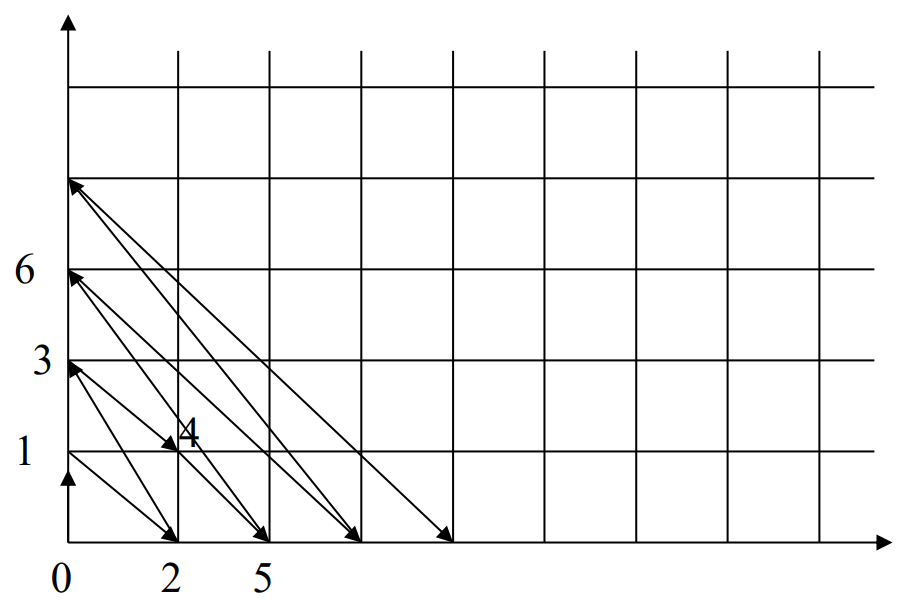
\includegraphics[width=8cm]{biiezione.png} 
    \caption{Grafico di biiezione}
  \end{figure}

  Si osservi che la funzione \(g(y,x)\) è computabile da una macchina di Turing, ossia \(\exists i\in \mathbb N : f_i=g\), ed è possibile calcolarla tramite i seguenti passaggi:
  \begin{enumerate}
    \item Si sceglie un alfabeto finito \(A\) per codificare i numeri naturali ed ogni altra informazione richiesta per la computazione;
    \item Si traduce la rappresentazione di \(n\) in un'opportuna rappresentazione della coppia \(<x,y>\) corrispondente ad \(n\). La rappresentazione decimale di \(n\) può essere tradotta nelle due rappresentazioni decimali di \(x\) ed \(y\), separate dal simbolo \(\$\);
    \item Si traduce \(y\) in un'opportuna codifica della TM \(y\)-esima \(M_y\) nella enumerazione di Gödel;
    \item Si simula la computazione di \(M_y\) su \(x\).
  \end{enumerate}

  \begin{theorem}
    Per ogni x ed ogni y, esiste e si può costruire una macchina di Turing universale in grado di calcolare \(g(y,x)=f_y(x)\)
  \end{theorem}  
  Tramite questo teorema si può affermare che è possibile creare una macchina di Turing che simuli il comportamento degli odierni calcolatori "general purpose".

  \section{Problemi Algoritmicamente Irrisolvibili}
  Come si è visto in precedenza, tutte le funzioni computabili \(f_y:\mathbb{N}\to\mathbb{N}\) si possono enumerare: questo significa che la cardinalità dell'insieme delle funzioni computabili è pari ad \(\aleph_0\), ovvero alla cardinalità dei numeri naturali \(\mathbb{N}\). L'insieme delle funzioni \(\{f:\mathbb{N}\to\mathbb{N}\}\) contiene la classe delle funzioni \(\{f:\mathbb{N}\to\{0,1\}\), in quanto \(\{0,1\}\subseteq \mathbb{N}\). Quindi, poichè \(\;|\;\{f:\mathbb{N}\to\mathbb{N}\}\;|\; \ge \;|\;\{f:\mathbb{N}\to\{0,1\}\}\;|\; = \wp (\mathbb{N}) = 2^{\aleph_0}\), si può dedurre che la cardinalità della classe delle funzioni da \(\mathbb{N}\) ad \(\mathbb{N}\) è strettamente maggiore della cardinalità della classe delle funzioni computabili: dunque, gran parte delle funzioni di \(\mathbb{N}\) non può essere calcolata. 

  Ora, quando si vuole definire una funzione si usa un linguaggio che la esprima, ovvero un sottoinsieme del monoide libero su di un determinato alfabeto finito: dunque, il linguaggio è un insieme numerabile. Si ricava quindi che la classe delle funzioni denotabili è a sua volta numerabile.

  Quando si scrive un programma, ci sono diverse proprietà che si vorebbero garantire. Una di queste è la terminazione del programma, ovvero la garanzia che, dato un qualsiasi ingresso conforme al programma stesso, esso termini la propria computazione e non vada, dunque, in un ciclo infinito. Nella realtà, però, non è possibile garantire a priori la terminazione del programma per un generico valore in ingresso, nè decidere atgtraverso un algoritmo se ciò possa avvenire in corrispondenza di uno specifico valore in ingresso. Più in generale, il problema della terminazione del calcolo automatico è in generale non decidibile, nonostante tale problema sia definibile.
  Si è quindi constatato che esistono problemi definibili, ma che non possono essere risolti algoritmicamente: dunque, l'insieme dei problemi definibili contiene strettamente l'insieme dei problemi risolvibili, nonostante entrambi siano numerabili e con la stessa cardinalità.

  \begin{figure}[!h]
    \begin{center}    
      \begin{tikzpicture}
        \foreach \X [count=\Y starting from 0.75] 
        in {\(f_y\) risolvibili, \(f\) definibili, \(f:\mathbb{N}\to\mathbb{N}\) (problemi totali)} {
          \draw (-\Y,-\Y/2) circle ({2*\Y} and \Y);
          \node at (1-2*\Y,-1.1*\Y) {\X}; 
        }
      \end{tikzpicture}
    \end{center}
    \caption{Gerarchia dei problemi}    
  \end{figure}

  \begin{theorem} [Halting Problem]
    Nessuna TM può calcolare la funzione \(g:\mathbb N\times \mathbb N \to \{0,1\}\) definita nel seguente modo:
    
    \(g(x,y) = if\; f_y(x) = \bot \; then \; 1 \; else \; 0\)
  \end{theorem}

  La dimostrazione di tale teorema si ottiene tramite la tecnica della diagonale, detta anche metodo di Cantor: l'obiettivo è quello di mostrare che un'enumerazione di oggetti di cardinalità almeno 2, non è completa, ossia che un oggetto che si vorrebbe trovare all'interno di tale enumerazione in realtà non è presente. L'enumerazione di una successione può essere rappresentata come una tabella con un numero infinito di righe. L'elemento che non compare in tale tabella viene individuato per assurdo considerando inizialmente la diagonale \(d\) (dunque \(d_i\) è l'elemento che si trova all'\(i\)-esima riga e all'\(i\)-esima colonna) e poi componendo una diagonale \(d'\) tale che, per ogni \(i\), \(d'_i\) sia diverso da \(d_i\).
  
  \begin{theorem}
    Nessuna TM è in grado di calcolare la funzione totale k definita nel seguente modo:

    \(k(x)= if\;f_x(x)\neq\bot\;then\;1\;else\;0\)
  \end{theorem}

  Questo problema rappresenta un caso speciale della funzione \(g(y,x)\) in quanto \(k(x)=g(x,x)\), dunque la calcolabilità della funzione \(k\) è direttamente correlata alla calcolabilità della funzione \(g\).
  Si noti che, in generale, se un problema è irrisolvibile, può accadere che un suo caso particolare sia risolvibile, mentre una sua generalizzazione è necessariamente irrisolvibile. Al contrario, se un problema è risolvibile, può accadere che una sua generalizzazione diventi irrisolvibile, mentre un suo caso particolare rimane sicuramente risolvibile.

  Un altro teorema certamente importante è il seguente:
  \begin{theorem}
    Nessuna TM è in grado di calcolare la funzione k definita nel seguente modo:

    \(k(y)=if\; f_y(x)\neq\bot\;then\;1\;else\;0\)
  \end{theorem}
  
  Da un punto di vista pratico questo problema è interessante perchè qualifica tutti i possibili dati in ingresso. Afferma, infatti, l'irrisolvibilità del problema di decidere se un certo programma termini la propria esecuzione per qualsiasi dato in ingresso o se, al contrario, per qualche dato il programma andrebbe in loop.Nel caso precedente, invece, si era interessati al problema di sapere se un certo programma con certi dati avrebbe terminato o meno la propria esecuzione.
  
  In definitiva, si è constatato che esistono problemi non risolvibili algoritmicamente. Ciò non esclude comunque la possibilità di trovare una soluzione per tali problemi, in quanto non tutti i problemi sono risolvibili tramite un procedimento algoritmico. 

  \section{Problemi di Decisione}
  Un problema di decisione è una domanda che ha come uniche risposte si o no (0, 1). Questo può anche essere espresso come un problema di appartenenza di un determinato elemento ad un certo insieme. Più in generale si noti che una qualsiasi proprietà di un determinato elemento di un insieme può essere formalizzata come un suo sottoinsieme (ad esempio, la proprietà di terminazione del calcolo per ogni valore dei dati in ingresso individua un sottoinsieme dell'insieme di tutti i programmi). 
  
  In questa sezione si prendono in particolare considerazione i sottoinsiemi di \(\mathbb N\), indicati convenzionalmente con \(S\subseteq\mathbb{N}\). Quindi, formalmente, dato un determinato elemento \(x\in\mathbb{N}\) e un insieme \(S\), si cerca di capire se \(x\) appartenga ad \(S\).

  \begin{definition}
    La funzione caratteristica \(c_S:\mathbb{N}\to\{0,1\}\) di un insieme S è definita come segue:

    \(c_S(x)=if\;x\in S\;then\;1\;else\;0\)
  \end{definition}

  La risolvibilità del problema di appartenenza ad un insieme (detta anche ricorsività dell'insieme) dipende dalla computabilità della funzione caratteristica \(c_S\), come definito di seguito:

  \begin{definition}
    Un insieme S è ricorsivo (o decidibile) se e solo se la sua funzione caratteristica è computabile.
  \end{definition}

  Si noti, inoltre, che per ogni insieme \(S\), la sua funzione caratteristica \(c_S\) è totale: infatti, dato un qualsiasi elemento \(x\in\mathbb{N}\), questo necessariamente apparteniene o non appartiene all'insieme.
  
  \begin{definition}
    Un insieme S è ricorsivamente enumerabile (o semidecidibile) se e solo se è l'insieme vuoto oppure è l'immagine di una funzione totale e computabile \(g_s\), ovvero:

    \(S=I_{g_s} = \{x\;|\;\exists y, y\in\mathbb{N} \land x=g_s(y)\}\)
  \end{definition}

  Gli insiemi decidibili devono il loro nome al fatto che il problema di appartenenza può essere risolto tramite un algoritmo meccanico e che, quindi, una TM che implementi la loro funzione caratteristica fornisce necessariamente una risposta al quesito se \(x\in S, \forall x \in \mathbb{N} \). Inoltre, per ogni insieme ricorsivamente numerabile \(S\) è possibile costruire una sequenza \(x_0=g_S(0), x_1=g_S(1), x_2=g_S(2),...\) tale per cui, se \(x\in S\), allora esiste \(i\) tale che \(x=g_S(i)\). In questo caso, esaminando la sequenza di elementi \(\{x_i\}\) si riuscirà a trovare l'elemento \(x\), concludendo che questo appartiene all'insieme \(S\). Perciò, se per un qualsiasi \(\bar{i}\) risultasse che \(x\notin\{g_S(i)\;|\;0\le i \le \bar{i}\}\) non si potrebbe concludere nè che \(x\in S\), nè che \(x\notin S\): per questo motivo, l'insieme \(S\) viene anche detto semidecidibile.

  \begin{theorem}
    Se S è ricorsivo, è anche ricorsivamente enumerabile. \\
    S è ricorsivo se e solo se sia S che \(\bar{S}=\mathbb{N}-S\) sono ricorsivamente enumerabili.
  \end{theorem}

  \break

  Quindi, riepilogando, si dice che un insieme \(S\) è:
  \begin{itemize}
    \item Ricorsivo (o Decidibile), se e solo se la sua funzione caratteristica \(c_S\) è computabile;
    \item Ricorsivamente enumerabile (o Semidecidibile), se e solo se:
    \begin{itemize}
      \item S è l'insieme vuoto;
      \item S è l'immagine di una funzione \(g_S\) totale e computabile (detta generatrice); \\ quindi, \(S=I_{g_S}=\{g_S(0), g_s(1), g_S(2),...\}\)
    \end{itemize}
  \end{itemize}

  Si consideri ora il seguente teorema:
  \begin{theorem}
    Per ogni insieme S, se \(i \in S\) implica che \(f_i\) sia totale e se per ogni funzione \(f\) totale e computabile, esiste \(i\in S\;|\;f=f_i\), allora S non è ricorsivamente enumerabile. 
  \end{theorem}

  Informalmente, questo teorema stabilisce che tutte le funzioni totali computabili non sono ricorsivamente enumerabili (mentre le funzioni parziali computabili lo sono). Dunque, tale teorema afferma implicitamente che non esiste nessun formalismo ricorsivamente enumerabile in grado di definire tutte e sole le funzioni totali e computabili: infatti, gli FSA sono in grado di definire le funzioni totali, ma non tutte, le TM definiscono tutte le funzioni computabili, ma anche quelle non totali, e un linguaggio di programmazione (come il C) è in grado di definire tutti gli algoritmi, ma anche anche quelli che non terminano mai. 
  
  Si cerca quindi di comprendere se sia possibile eliminare le funzioni non totali: per far ciò, si prenda in considerazione una generica funzione parziale, ad esempio, arricchendo \(\mathbb{N}\) con il valore \(\{\bot\}\) o con qualsiasi altro simbolo che indichi che la funzione non è definita per certi valori. Tale trasformazione da funzione parziale a totale, però, non può essere applicata perchè nel passaggio è possibile perdere la computabilità della funzione. Questo risultato è enunciato nel seguente teorema:
  
  \begin{theorem}
    Non esiste una funzione totale e computabile h che sia un'estensione della seguente funzione:
    \(g(x)=if\;f_x(x)\neq\bot\;then\;f_x(x)+1\;else\;\bot\)
  \end{theorem}

  Tale teorema, afferma quindi che non è possibile estendere una funzione parziale ad una totale, in quanto si potrebbe perdere la sua computabilità.

  Vale anche il seguente risultato:
  \begin{theorem}
    Un insieme S è ricorsivamente enumerabile se e solo se \(S=D_h\), in cui h è una funzione parziale e computabile (\(S=\{x\;|\;h(x)\neq \bot\}\)), oppure se e solo se \(S=I_g\), in cui g è una funzione parziale e computabile (\(S=\{x\;|\;x=g(y), y\in \mathbb{N}\}\)).
  \end{theorem}

  Quindi, dato l'insieme \(K=\{x\;|\;f(x) \neq \bot\}\) questo è semidecidibile perchè \(K=D_h\), con \(h(x)=f_x(x)\), ma è anche indecidibile in quanto la funzione caratteristica dell'insieme \(K\), definita come \(c_K(x)=if\;f_x(x)\neq \bot\;then\;1\;else\;0\), non è computabile. Si è appena dimostrato che esistono insiemi che sono semidecidibili, ma allo stesso tempo indecidibili.

  \begin{figure}[!h]
    \begin{center}    
      \begin{tikzpicture}
        \foreach \X [count=\Y starting from 0.75] 
        in {insiemi ricorsivi, insiemi RE*, \(\wp(\mathbb{N})\)} {
          \draw (-\Y,-\Y/2) circle ({2*\Y} and \Y);
          \node at (1-2*\Y,-1.1*\Y) {\X}; 
        }
      \end{tikzpicture}
    \end{center}
    \caption{Gerarchia degli insiemi}    
  \end{figure}

  *Con RE si indicano gli insiemi Ricorsivamente Enumerabili.

  Si noti che tutte le inclusioni sono strette.

  \section{Teoremi di Kleene e Rice}

  \begin{theorem} [Teorema di Kleene del punto fisso]
    Sia t una qualunque funzione totale e computabile. Allora è sempre possibile trovare un intero p, tale per cui:
    
    \(f_p=f_{t(p)}\)\\
    La funzione \(f_p\) è detta punto fisso di t, perchè t trasforma \(f_p\) in \(f_p\) stessa.
  \end{theorem}

  \begin{theorem}[Teorema di Rice]
    Sia F un insieme generico di funzioni computabili. L'insieme \(S=\{x\;|\;f_x\in F\}\) degli indici delle TM che calcolano le funzioni di F, è ricorsivo se e solo se \(F=\emptyset\) oppure F è l'insieme di tutte le funzioni computabili.
  \end{theorem}

  Il teorema di Rice ha un forte impatto pratico negativo, in quanto afferma che. in tutti i casi non banali, \(S\) non è decidibile. Non è quindi possibile stabilire algoritmicamente se un dato algoritmo sia in grado di risolvere un determinato problema, nè se due programmi siano equivalenti (ossia se calcolino la stessa funzione). Il grande impatto pratico del teorema di Rice deriva dal fatto che il concetto di sottoinsieme \(F\) di funzioni computabili è un'espressione formale del concetto generale di proprietà di problemi risolvibili: una proprietà degli elementi di un insieme è un sottoinsieme dell'insieme dato e una funzione computabile è una formalizzazione del concetto di problema risolvibile; quindi, il teorema di Rice efferma che non è possibile stabilire se un determinato algoritmo risolve un problema pur risolvibile che godia di una qualsiasi proprietà non banale.
  \chapter{Computabilità}
  In questa sezione si cercherà di rispondere alla domanda: quali problemi possono essere affrontati e risolti mediante gli automi analizzati?
  Si ricordi che automi e grammatiche, pur essendo modelli matematici, si possono considerare dispositivi meccanici per la risoluzione di problemi e che esistono formalismi che hanno un potere espressivo maggiore di altri, ossia sono in grado di riconoscere una classe di linguaggi che altri formalismi non riescono a riconoscere. Inoltre, si ricordi che, nessun formalismo è più potente delle macchine di Turing, sia dal punto di vista del riconoscimento che della traduzione di linguaggi e, per tanto, sono detti formalismi massimi.

  \section{Formalizzazione dei Problemi}
  Molti problemi possono essere opportunamente descritti come il riconoscimento di un determinato linguaggio o come la sua traduzione in un altro linguaggio. Ogni problema matematico è descrivibile mediante una di queste forme, alla sola condizione che il dominio di tale problema sia un insieme numerabile, in maniera tale che i suoi elementi si possono porre in corrispondenza biunivoca con gli elementi di \(\mathbb N\) o, se si preferisce, di \(V^*\), in cui \(V\) rappresenta un alfabeto. Dunque, il problema di origine si può riformulare come il problema di calcolo di una funzione \(f:\mathbb N\to\mathbb N\). Quanto detto è in perfetto accordo con tutti i formalismi matematici esaminati fino ad ora: questi, infatti, sono discreti e hanno un dominio matematico numerabile.

  Il riconoscimento di linguaggi e la loro traduzione sono due formulazioni differenti di un problema, che sono facilmente riducibili l'uno all'altro. Infatti, il problema di stabilire se una determinata stringa \(x\) appartenga o meno al linguaggio \(L\) può anche essere impostato come la traduzione \(\tau_L(x)\), per cui \(\tau_L(x) = 1\) se \(x\in L\), \(\tau_L(x)=0\) altrimenti. Viceversa, data la traduzione \(\tau:V_1^*\to V_2^*\), si può definire il linguaggio seguente:
  
  \(L_{\tau}=\{z\;|\;z=x\$y,\; x\in V_1^*,\; y=\tau(x)\in V_2^*,\; \$ \notin (V_1\cup V_2)\} \)
  
  \noindent ovvero il linguaggio formato da una stringa e la sua traduzione, separati dal simbolo \(\$\). Un dispositivo che riconosce il linguaggio \(L_{\tau}\) può essere utilizzato come trasduttore che calcola \(\tau\): per ogni \(x\), infatti, è possibile enumerare tutte le \(y\in V_2^*\) e verificare se \(x\$y\in L_{\tau}\) oppure no. Prima o poi, se la funzione \(\tau(x)\neq \bot \), verrà trovata una stringa per cui la macchina risponderà positivamente.

  \section{Tesi di Church}
  Le macchine di Turing, come visto in precedenza, sono il formalismo più potente che si ha a disposizione per il calcolo computazionale: ogni programma eseguibile da un calcolatore moderno può essere eseguito anche da una macchina di Turing. Dunque, le macchine di Turing hanno la stessa espressività dei linguaggi di programmazione ad alto livello, detti anche Turing completi. 

  Più formalmente, data una TM M, è possibile costruire un programma, scritto in un determinato linguaggio di programmazione (come C, Java ecc...), che simuli il comportamento di M, purchè il calcolatore disponga di una quantità di memoria sufficiente durante l'esecuzione. Inoltre, dato un programma scritto in un determinato linguaggio di programmazione, è possibile costruire una TM M che calcoli la stessa funzione calcolata dal programma.

  \begin{thesis}[Tesi di Church - Prima Parte]
    Non esiste alcun formalismo, per modellare una determinata computazione meccanica, che sia più potente delle TM e dei formalismi ad essi equivalenti.
  \end{thesis}

  La tesi di Church non è un teorema perchè per sua natura non è dimostrabile, in quanto andrebbe verificato ogni qual volta si introduce un nuovo formalismo computazionale.

  In base a questo risultato si può affermare che, se si riesce a dimostrare che un determinato problema è risolvibile da una TM, allora è sicuramente possibile risolverlo mediante un modello matematico di calcolo, che abbia la stessa potenza delle macchine di Turing. Viceversa, se si dimostra che un problema non può essere risolto da una TM, allora è verificato che tale problema è irrisolvibile da qualunque modello matematico.

  \paragraph{Algoritmi}
  Si introduce ora il concetto di algoritmo, centrale nell'informatica. Per algoritmo si intende la procedura di risoluzione di un problema mediante un dispositivo automatico di calcolo. Gli algoritmi si possono anche intendere come un metodo astratto di descrizione dei programmi eseguibili, ovvero una sequenza di comandi che, una volta eseguiti, portano alla risoluzione del problema.
  
  Ogni algoritmo ha le seguenti proprietà:
  \begin{enumerate}
    \item Un algoritmo deve contenere una sequenza finita di istruzioni;
    \item Ogni istruzione deve essere immediatamente eseguibile da qualche procedimento meccanico di calcolo, ossia deve esistere un processore che sia in grado di comprendere univocamente le istruzioni e di eseguirle producendo risultati precisi ed inequivocabili;
    \item Il processore è dotato di celle di memoria in cui possono essere immagazzinati i riultati intermedi;
    \item La computazione è discreta, ossia l'informazione è codificata in forma digitale e la computazione procede attraverso passi discreti;
    \item Gli algoritmi vengono eseguiti deterministicamente;
    \item Non esiste un limite finito sui dati di ingresso e di uscita: ogni calcolatore può ricevere in ingresso o emettere in uscita stringhe di lunghezza arbitraria;
    \item Non esiste un limite alla quantità di memoria richiesta per effettuare i calcoli;
    \item Non esiste un limite al numero di passi discreti richiesti per effettuare un calcolo ed è dunque possibile avere computazioni infinite.
  \end{enumerate}

  La tesi di Church non si ferma solo nell'affermazione che nessun formalismo sia più espressivo delle TM, ma afferma anche che nessun algoritmo è in grado di risolvere un problema che non è risolvibile da una TM. Formalmente:

  \begin{thesis}[Tesi di Church - Seconda Parte]
    Ogni algoritmo per la soluzione automatica di un problema può essere codificato in termini di una TM (o di un formalismo a potenza equivalente).
  \end{thesis}

  \begin{theorem}
    Ogni funzione (o problema), per cui esiste una TM che la calcoli (o risolva), si dice computabile o calcolabile (o risolvibile). Un problema risolvibile la cui risposta sia booleana ed esistente per ogni valore del dominio di definizione (ossia è formalizzato da una funzione calcolabile e totale) si dice decidibile.
  \end{theorem}

  Grazie alla seconda parte della tesi di Church si può affermare che è possibile studiare i limiti del calcolo automatico indipendentemente dalla formalizzazione del problema e del particolare modello computazionale.

  \section{Enumerazione delle TM}
  Le macchine di Turing possono essere viste come dei calcolatori astratti, specializzati nella risoluzione di un solo problema e non programmabili. Ci si pone quindi la domanda: 'le TM sono in grado di simulare i calcolatori programmabili e di risolvere i problemi da \(\mathbb{N}\) a \(\mathbb{N}\)?'

  Per poter rispondere a tale domanda, si noti innanzitutto che dato un qualsiasi insieme S, questo può essere enumerato algoritmicamente se è possibile stabilire una biiezione fra l'insieme \(S\) e l'insieme dei numeri naturali \(\mathbb{N}\), calcolabile attraverso un algoritmo o da una TM.
  Alla stessa maniera è possibile enumerare algoritmicamente l'insieme delle TM tramite una biiezione \(E:\{TM\}\leftrightarrow\mathbb{N}\). Tale biiezione è implementabile da un algoritmo che riceve in ingresso un numero \(n\) e ritorna la \(n\)-esima macchina di Turing. Un'enumerazione calcolabile da una TM viene chiamata Gödelizzazione, mentre il numero naturale biiettivamente associato da tale enumerazione ad una TM è detto numero di Gödel della TM. 

  Inoltre, è noto che una TM M può risolvere una funzione \(f_M:D\to R\), con \(D\) ed \(R\) opportunamente codificati nell'alfabeto di \(M\), dunque si indicherà con \(f_y\) la funzione calcolata dalla \(y\)-esima macchina di Turing, indicata con \(M_y=E(y)\).

  \section{Macchine di Turing Universali}
  Le UTM (Universal Turing Machines) sono TM in grado di modellare dispositivi generali di risoluzione dei problemi, in cui il problema da risolvere non viene codificato nella struttura del dispositivo (come avviene per le TM), ma gli viene fornito come input, assieme ai dati con cui operare (esattamente come gli odierni calcolatori). Le UTM sono quindi MT che calcolano la funzione \(g(y,x)=f_y(x)\), in cui \(y\) rappresenta la funzione \(f_y\), calcolata dalla TM \(M_y\), ed \(x\) rappresenta l'ingresso su cui \(M_y\) opera; calcolano, dunque, il valore della funzione \(f_y\) applicata ad \(x\).

  Come si può osservare, la UTM così definita non sembra appartenere all'insieme delle macchine di Turing, in quanto la funzione \(g(y,x)\) è opera da \(\mathbb{N}\times\mathbb{N}\) ad \(\mathbb{N}\), anzichè da \(\mathbb{N}\) ad \(\mathbb{N}\) come tutte le altre TM. È però possibile, come già dimostrato in precedenza, definire una biiezione calcolabile algoritmicamente, tramite la funzione:
  \begin{equation*}
    \displaystyle d(x,y) = x+\frac{(x+y)(x+y-1)}{2}
  \end{equation*}
  che mette in corrispondenza l'insieme \(\mathbb{N}\times\mathbb{N}\), composto dalle coppie di numeri naturali, all'insieme \(\mathbb{N}\), composto da numeri naturali.

  Graficamente, è come visitare le coppie di punti nel piano in un ordine prefissato, dove la posizione di un punto nella visita rappresenta il numero naturale associato alla coppia che identifica le coordinate del punto.
  
  \begin{figure}[!h]
    \centering
    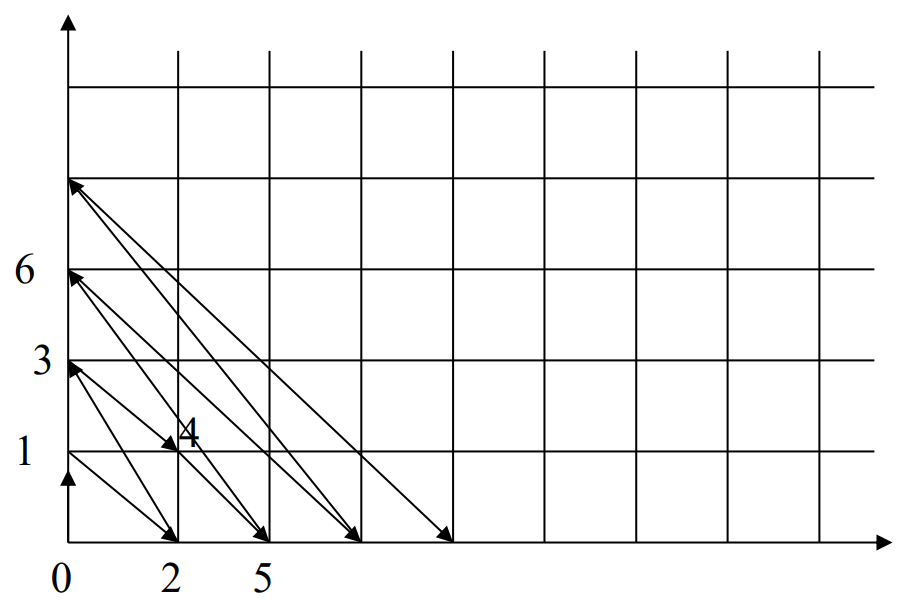
\includegraphics[width=8cm]{biiezione.png} 
    \caption{Grafico di biiezione}
  \end{figure}

  Si osservi che la funzione \(g(y,x)\) è computabile da una macchina di Turing, ossia \(\exists i\in \mathbb N : f_i=g\), ed è possibile calcolarla tramite i seguenti passaggi:
  \begin{enumerate}
    \item Si sceglie un alfabeto finito \(A\) per codificare i numeri naturali ed ogni altra informazione richiesta per la computazione;
    \item Si traduce la rappresentazione di \(n\) in un'opportuna rappresentazione della coppia \(<x,y>\) corrispondente ad \(n\). La rappresentazione decimale di \(n\) può essere tradotta nelle due rappresentazioni decimali di \(x\) ed \(y\), separate dal simbolo \(\$\);
    \item Si traduce \(y\) in un'opportuna codifica della TM \(y\)-esima \(M_y\) nella enumerazione di Gödel;
    \item Si simula la computazione di \(M_y\) su \(x\).
  \end{enumerate}

  \begin{theorem}
    Per ogni x ed ogni y, esiste e si può costruire una macchina di Turing universale in grado di calcolare \(g(y,x)=f_y(x)\)
  \end{theorem}  
  Tramite questo teorema si può affermare che è possibile creare una macchina di Turing che simuli il comportamento degli odierni calcolatori "general purpose".

  \section{Problemi Algoritmicamente Irrisolvibili}
  Come si è visto in precedenza, tutte le funzioni computabili \(f_y:\mathbb{N}\to\mathbb{N}\) si possono enumerare: questo significa che la cardinalità dell'insieme delle funzioni computabili è pari ad \(\aleph_0\), ovvero alla cardinalità dei numeri naturali \(\mathbb{N}\). L'insieme delle funzioni \(\{f:\mathbb{N}\to\mathbb{N}\}\) contiene la classe delle funzioni \(\{f:\mathbb{N}\to\{0,1\}\), in quanto \(\{0,1\}\subseteq \mathbb{N}\). Quindi, poichè \(\;|\;\{f:\mathbb{N}\to\mathbb{N}\}\;|\; \ge \;|\;\{f:\mathbb{N}\to\{0,1\}\}\;|\; = \wp (\mathbb{N}) = 2^{\aleph_0}\), si può dedurre che la cardinalità della classe delle funzioni da \(\mathbb{N}\) ad \(\mathbb{N}\) è strettamente maggiore della cardinalità della classe delle funzioni computabili: dunque, gran parte delle funzioni di \(\mathbb{N}\) non può essere calcolata. 

  Ora, quando si vuole definire una funzione si usa un linguaggio che la esprima, ovvero un sottoinsieme del monoide libero su di un determinato alfabeto finito: dunque, il linguaggio è un insieme numerabile. Si ricava quindi che la classe delle funzioni denotabili è a sua volta numerabile.

  Quando si scrive un programma, ci sono diverse proprietà che si vorrebbero garantire. Una di queste è la terminazione del programma, ovvero la garanzia che, dato un qualsiasi ingresso conforme al programma stesso, esso termini la propria computazione e non vada, dunque, in un ciclo infinito. Nella realtà, però, non è possibile garantire a priori la terminazione del programma per un generico valore in ingresso, nè decidere attraverso un algoritmo se ciò possa avvenire in corrispondenza di uno specifico valore in ingresso. Più in generale, il problema della terminazione del calcolo automatico è in generale non decidibile, nonostante tale problema sia definibile.
  Si è quindi constatato che esistono problemi definibili, ma che non possono essere risolti algoritmicamente: dunque, l'insieme dei problemi definibili contiene strettamente l'insieme dei problemi risolvibili, nonostante entrambi siano numerabili e con la stessa cardinalità.

  \begin{figure}[!h]
    \begin{center}    
      \begin{tikzpicture}
        \foreach \X [count=\Y starting from 0.75] 
        in {\(f_y\) risolvibili, \(f\) definibili, \(f:\mathbb{N}\to\mathbb{N}\) (problemi totali)} {
          \draw (-\Y,-\Y/2) circle ({2*\Y} and \Y);
          \node at (1-2*\Y,-1.1*\Y) {\X}; 
        }
      \end{tikzpicture}
    \end{center}
    \caption{Gerarchia dei problemi}    
  \end{figure}

  \begin{theorem} [Halting Problem]
    Nessuna TM può calcolare la funzione \(g:\mathbb N\times \mathbb N \to \{0,1\}\) definita nel seguente modo:
    
    \(g(x,y) = if\; f_y(x) = \bot \; then \; 1 \; else \; 0\)
  \end{theorem}

  La dimostrazione di tale teorema si ottiene tramite la tecnica della diagonale, detta anche metodo di Cantor: l'obiettivo è quello di mostrare che un'enumerazione di oggetti di cardinalità almeno 2, non è completa, ossia che un oggetto che si vorrebbe trovare all'interno di tale enumerazione in realtà non è presente. L'enumerazione di una successione può essere rappresentata come una tabella con un numero infinito di righe. L'elemento che non compare in tale tabella viene individuato per assurdo considerando inizialmente la diagonale \(d\) (dunque \(d_i\) è l'elemento che si trova all'\(i\)-esima riga e all'\(i\)-esima colonna) e poi componendo una diagonale \(d'\) tale che, per ogni \(i\), \(d'_i\) sia diverso da \(d_i\).
  
  \begin{theorem}
    Nessuna TM è in grado di calcolare la funzione totale k definita nel seguente modo:

    \(k(x)= if\;f_x(x)\neq\bot\;then\;1\;else\;0\)
  \end{theorem}

  Questo problema rappresenta un caso speciale della funzione \(g(y,x)\) in quanto \(k(x)=g(x,x)\), dunque la calcolabilità della funzione \(k\) è direttamente correlata alla calcolabilità della funzione \(g\).
  Si noti che, in generale, se un problema è irrisolvibile, può accadere che un suo caso particolare sia risolvibile, mentre una sua generalizzazione è necessariamente irrisolvibile. Al contrario, se un problema è risolvibile, può accadere che una sua generalizzazione diventi irrisolvibile, mentre un suo caso particolare rimane sicuramente risolvibile.

  Un altro teorema certamente importante è il seguente:
  \begin{theorem}
    Nessuna TM è in grado di calcolare la funzione k definita nel seguente modo:

    \(k(y)=if\; f_y(x)\neq\bot\;then\;1\;else\;0\)
  \end{theorem}
  
  Da un punto di vista pratico questo problema è interessante perchè qualifica tutti i possibili dati in ingresso. Afferma, infatti, l'irrisolvibilità del problema di decidere se un certo programma termini la propria esecuzione per qualsiasi dato in ingresso o se, al contrario, per qualche dato il programma andrebbe in loop. Nel caso precedente, invece, si era interessati al problema di sapere se un certo programma con certi dati avrebbe terminato o meno la propria esecuzione.
  
  In definitiva, si è constatato che esistono problemi non risolvibili algoritmicamente. Ciò non esclude comunque la possibilità di trovare una soluzione per tali problemi, in quanto non tutti i problemi sono risolvibili tramite un procedimento algoritmico. 

  \section{Problemi di Decisione}
  Un problema di decisione è una domanda che ha come uniche risposte si o no (0, 1). Questo può anche essere espresso come un problema di appartenenza di un determinato elemento ad un certo insieme. Più in generale si noti che una qualsiasi proprietà di un determinato elemento di un insieme può essere formalizzata come un suo sottoinsieme (ad esempio, la proprietà di terminazione del calcolo per ogni valore dei dati in ingresso individua un sottoinsieme dell'insieme di tutti i programmi). 
  
  In questa sezione si prendono in particolare considerazione i sottoinsiemi di \(\mathbb N\), indicati convenzionalmente con \(S\subseteq\mathbb{N}\). Quindi, formalmente, dato un determinato elemento \(x\in\mathbb{N}\) e un insieme \(S\), si cerca di capire se \(x\) appartenga ad \(S\).

  \begin{definition}
    La funzione caratteristica \(c_S:\mathbb{N}\to\{0,1\}\) di un insieme S è definita come segue:

    \(c_S(x)=if\;x\in S\;then\;1\;else\;0\)
  \end{definition}

  La risolvibilità del problema di appartenenza ad un insieme (detta anche ricorsività dell'insieme) dipende dalla computabilità della funzione caratteristica \(c_S\), come definito di seguito:

  \begin{definition}
    Un insieme S è ricorsivo (o decidibile) se e solo se la sua funzione caratteristica è computabile.
  \end{definition}

  Si noti, inoltre, che per ogni insieme \(S\), la sua funzione caratteristica \(c_S\) è totale: infatti, dato un qualsiasi elemento \(x\in\mathbb{N}\), questo necessariamente appartiene o non appartiene all'insieme.
  
  \begin{definition}
    Un insieme S è ricorsivamente enumerabile (o semidecidibile) se e solo se è l'insieme vuoto oppure è l'immagine di una funzione totale e computabile \(g_s\), ovvero:

    \(S=I_{g_s} = \{x\;|\;\exists y, y\in\mathbb{N} \land x=g_s(y)\}\)
  \end{definition}

  Gli insiemi decidibili devono il loro nome al fatto che il problema di appartenenza può essere risolto tramite un algoritmo meccanico e che, quindi, una TM che implementi la loro funzione caratteristica fornisce necessariamente una risposta al quesito se \(x\in S, \forall x \in \mathbb{N} \). Inoltre, per ogni insieme ricorsivamente numerabile \(S\) è possibile costruire una sequenza \(x_0=g_S(0), x_1=g_S(1), x_2=g_S(2),...\) tale per cui, se \(x\in S\), allora esiste \(i\) tale che \(x=g_S(i)\). In questo caso, esaminando la sequenza di elementi \(\{x_i\}\) si riuscirà a trovare l'elemento \(x\), concludendo che questo appartiene all'insieme \(S\). Perciò, se per un qualsiasi \(\bar{i}\) risultasse che \(x\notin\{g_S(i)\;|\;0\le i \le \bar{i}\}\) non si potrebbe concludere nè che \(x\in S\), nè che \(x\notin S\): per questo motivo, l'insieme \(S\) viene anche detto semidecidibile.

  \begin{theorem}
    Se S è ricorsivo, è anche ricorsivamente enumerabile. \\
    S è ricorsivo se e solo se sia S che \(\bar{S}=\mathbb{N}-S\) sono ricorsivamente enumerabili.
  \end{theorem}

  \break

  Quindi, riepilogando, si dice che un insieme \(S\) è:
  \begin{itemize}
    \item Ricorsivo (o Decidibile), se e solo se la sua funzione caratteristica \(c_S\) è computabile;
    \item Ricorsivamente enumerabile (o Semidecidibile), se e solo se:
    \begin{itemize}
      \item S è l'insieme vuoto;
      \item S è l'immagine di una funzione \(g_S\) totale e computabile (detta generatrice); \\ quindi, \(S=I_{g_S}=\{g_S(0), g_s(1), g_S(2),...\}\)
    \end{itemize}
  \end{itemize}

  Si consideri ora il seguente teorema:
  \begin{theorem}
    Per ogni insieme S, se \(i \in S\) implica che \(f_i\) sia totale e se per ogni funzione \(f\) totale e computabile, esiste \(i\in S\;|\;f=f_i\), allora S non è ricorsivamente enumerabile. 
  \end{theorem}

  Informalmente, questo teorema stabilisce che tutte le funzioni totali computabili non sono ricorsivamente enumerabili (mentre le funzioni parziali computabili lo sono). Dunque, tale teorema afferma implicitamente che non esiste nessun formalismo ricorsivamente enumerabile in grado di definire tutte e sole le funzioni totali e computabili: infatti, gli FSA sono in grado di definire le funzioni totali, ma non tutte, le TM definiscono tutte le funzioni computabili, ma anche quelle non totali, e un linguaggio di programmazione (come il C) è in grado di definire tutti gli algoritmi, ma anche quelli che non terminano mai. 
  
  Si cerca quindi di comprendere se sia possibile eliminare le funzioni non totali: per far ciò, si prenda in considerazione una generica funzione parziale, ad esempio, arricchendo \(\mathbb{N}\) con il valore \(\{\bot\}\) o con qualsiasi altro simbolo che indichi che la funzione non è definita per certi valori. Tale trasformazione da funzione parziale a totale, però, non può essere applicata perchè nel passaggio è possibile perdere la computabilità della funzione. Questo risultato è enunciato nel seguente teorema:
  
  \begin{theorem}
    Non esiste una funzione totale e computabile h che sia un'estensione della seguente funzione:
    \(g(x)=if\;f_x(x)\neq\bot\;then\;f_x(x)+1\;else\;\bot\)
  \end{theorem}

  Tale teorema, afferma quindi che non è possibile estendere una funzione parziale ad una totale, in quanto si potrebbe perdere la sua computabilità.

  Vale anche il seguente risultato:
  \begin{theorem}
    Un insieme S è ricorsivamente enumerabile se e solo se \(S=D_h\), in cui h è una funzione parziale e computabile (\(S=\{x\;|\;h(x)\neq \bot\}\)), oppure se e solo se \(S=I_g\), in cui g è una funzione parziale e computabile (\(S=\{x\;|\;x=g(y), y\in \mathbb{N}\}\)).
  \end{theorem}

  Quindi, dato l'insieme \(K=\{x\;|\;f(x) \neq \bot\}\) questo è semidecidibile perchè \(K=D_h\), con \(h(x)=f_x(x)\), ma è anche indecidibile in quanto la funzione caratteristica dell'insieme \(K\), definita come \(c_K(x)=if\;f_x(x)\neq \bot\;then\;1\;else\;0\), non è computabile. Si è appena dimostrato che esistono insiemi che sono semidecidibili, ma allo stesso tempo indecidibili.

  \begin{figure}[!h]
    \begin{center}    
      \begin{tikzpicture}
        \foreach \X [count=\Y starting from 0.75] 
        in {insiemi ricorsivi, insiemi RE*, \(\wp(\mathbb{N})\)} {
          \draw (-\Y,-\Y/2) circle ({2*\Y} and \Y);
          \node at (1-2*\Y,-1.1*\Y) {\X}; 
        }
      \end{tikzpicture}
    \end{center}
    \caption{Gerarchia degli insiemi}    
  \end{figure}

  *Con RE si indicano gli insiemi Ricorsivamente Enumerabili.

  Si noti che tutte le inclusioni sono strette.

  \section{Teoremi di Kleene e Rice}

  \begin{theorem} [Teorema di Kleene del punto fisso]
    Sia t una qualunque funzione totale e computabile. Allora è sempre possibile trovare un intero p, tale per cui:
    
    \(f_p=f_{t(p)}\)\\
    La funzione \(f_p\) è detta punto fisso di t, perchè t trasforma \(f_p\) in \(f_p\) stessa.
  \end{theorem}

  \begin{theorem}[Teorema di Rice]
    Sia F un insieme generico di funzioni computabili. L'insieme \(S=\{x\;|\;f_x\in F\}\) degli indici delle TM che calcolano le funzioni di F, è ricorsivo se e solo se \(F=\emptyset\) oppure F è l'insieme di tutte le funzioni computabili.
  \end{theorem}

  Il teorema di Rice ha un forte impatto pratico negativo, in quanto afferma che, in tutti i casi non banali, \(S\) non è decidibile. Non è quindi possibile stabilire algoritmicamente se un dato algoritmo sia in grado di risolvere un determinato problema, nè se due programmi siano equivalenti (ossia se calcolino la stessa funzione). Il grande impatto pratico del teorema di Rice deriva dal fatto che il concetto di sottoinsieme \(F\) di funzioni computabili è un'espressione formale del concetto generale di proprietà di problemi risolvibili: una proprietà degli elementi di un insieme è un sottoinsieme dell'insieme dato e una funzione computabile è una formalizzazione del concetto di problema risolvibile; quindi, il teorema di Rice afferma che non è possibile stabilire se un determinato algoritmo risolve un problema pur risolvibile che godi di una qualsiasi proprietà non banale.

  \part{Algoritmi e Strutture Dati}
  \chapter{Complessità del Calcolo}
  Nei capitoli precedenti si è dimostrato come esistano alcuni problemi che, pur essendo ben definiti, non sono risolvibili algoritmicamente, per cui non esiste una TM in grado di risolvere quel determinato problema. Un'altra difficoltà da tenere in considerazione quando si manipolano i problemi, risiede nel tempo di esecuzione, ovvero il tempo impiegato dal programma per fornire una soluzione: se non è possibile ottenere una soluzione in un tempo ragionevole, ovviamente, il problema diventa intrattabile, nonostante sia teoricamente risolvibile.

  Il concetto di intrattabilità è strettamente correlato al concetto di complessità del calcolo: più il problema è complesso e meno questo diventa trattabile. Informalmente, la complessità indica una misura del prezzo da pagare per risolvere il problema. Le risorse che si utilizzano per la risoluzione di un problema sono principalmente due: lo spazio, ovvero la memoria necessaria all'algoritmo, e il tempo richiesto per produrre la soluzione. Si parlerà quindi di complessità spaziale e di complessità temporale.

  Si osservi inoltre che le due risorse, quella temporale e quella spaziale, seppur sembrino indipendenti l'una dall'altra, sono in realtà correlate: alla riduzione di utilizzo di una risorsa aumenta l'altra e viceversa. 

  \section{Analisi di complessità}
  La complessità del calcolo dipende dalla dimensione e, spesso, anche dai particolari valori assunti dai dati in ingresso. Per questo motivo, si rende necessario effettuare un'analisi del caso pessimo, del caso medio e del caso ottimo, in funzione della dimensione dei dati in ingresso. Più formalmente, tali casi rappresentano rispettivamente la scelta di ingressi per cui viene eseguito il massimo numero di istruzioni nel programma, il comportamento del programma in relazione alla possibile distribuzione dei dati e la scelta di input per cui viene eseguito il minor numero di istruzioni.

  In generale, il caso ottimo non è di particolare interesse e il caso medio richiede la conoscenza della distribuzione dei dati in ingresso (non sempre nota). Il caso pessimo, invece, è particolarmente interessante in quanto fornisce i peggiori risultati ottenibili dall'algoritmo in termini di consumo di spazio o tempo; si garantisce quindi che tutte le soluzioni proposte dall'algoritmo abbiano un dispendio di risorse minore rispetto al caso pessimo, indipendentemente dalla tipologia degli ingressi. Dunque, se il caso pessimo è ritenuto accettabile, allora anche tutti gli altri casi lo sono. 

  Inoltre, a differenza di quanto analizzato per la risolvibilità dei problemi, la complessità non è collegata solo al problema che si vuole affrontare, ma dipende anche dell'algoritmo che si utilizza per risolverlo. 

  \paragraph{}
  Nel capitolo sugli automi, è stato più volte affermato che le Macchine di Turing sono il formalismo più potente che si ha a disposizione per la risoluzione di problemi, dunque, risulta ragionevole definire la complessità temporale e spaziale impiegando un tale modello.

  \begin{definition} \label{complessita temporale} 
    Sia \(M\) una TM deterministica a \(k\) nastri e sia \(x\in I^*\). Sia \(c_0\vdash c_1\vdash....\vdash c_r\) una computazione, ovvero una sequenza di transizioni di \(M\) tale che \(c_0=<q_0,\;\!\uparrow\! x,\; \!\uparrow\! Z_0,\; ...,\; \!\uparrow\! Z_0>\) e \\ \(c_i=<q_i,\;x_i\!\uparrow\! y_i,\; \alpha_{i1}\!\uparrow\! \beta_{i1},\; ...,\; \alpha_{ik}\!\uparrow\! \beta_{ik}>\), in cui \(c_r\) è una configurazione di arresto, se esiste. Allora, la funzione che rappresenta la complessità temporale \({T}_M\) di \(M\) è definita nel seguente modo:
    \begin{equation*}
      {T}_M=if\;la\;computazione\;termina\;then\;r\;else\;\infty.
    \end{equation*}
  \end{definition}

  Informalmente, quindi, la complessità temporale viene definita come una funzione che fornisce il numero esatto di passi richiesti da una TM per raggiungere la propria configurazione di arresto, se esiste, a partire dalla configurazione iniziale, per una qualsiasi stringa in ingresso. analogamente, si può definire la complessità spaziale come una funzione che fornisce il numero massimo di celle del nastro utilizzate.

  \begin{definition} \label{complessita spaziale}
    Siano M, x, \(c_0,...,c_r\) definiti come nella definizione \ref{complessita temporale}. La funzione che rappresenta la complessità spaziale \({S}_M\) di M è definita nel seguente modo:

    \begin{equation*}
      \displaystyle {S}_M=\sum_{j=1}^{k} max_{i\in\{0,1,...,r\}}(|\alpha_{ij}|)
    \end{equation*}
    Inoltre, vale che:
    \begin{equation*}
      \forall x, \frac{{S}_M}{k}\le {T}_M(x)
    \end{equation*}
  \end{definition}

  Si noti, inoltre, che la definizione di \({S}_M(x)\) prende in considerazione solamente i nastri di memoria e ignora sia il nastro di ingresso che il nastro di uscita per il calcolo della complessità.

  Secondo le definizioni \ref{complessita temporale} e \ref{complessita spaziale}, sia \({T}_M\) che \({S}_M\) sono funzioni definite su \(I^*\), ma nella pratica la complessità di una soluzione dipende sia dal contenuto dell'ingresso che dalla sua dimensione: a partire da questa osservazione, si erano introdotti i concetti di complessità nel caso pessimo, medio e ottimo, che si possono ridefinire nel seguente modo, alla luce delle definizioni appena date:

  \begin{definition}
    Il caso pessimo, ottimo e medio sono così definiti:
    \begin{itemize}
      \item Caso pessimo: \({T}_M(n)=max_{|x|=n}{T}_M(x)\);
      \item Caso ottimo: \({T}_M(n)=min_{|x|=n}{T}_M(x)\);
      \item Caso medio: \(\displaystyle {T}_M(n)=\frac{\sum_{|x|=n}{T}_M(x)}{|I|^n}\)
    \end{itemize}
  \end{definition}

  Una volta analizzata la complessità temporale tramite il formalismo delle macchine di Turing, si sposta l'attenzione sugli altri formalismi analizzati nel capitolo riguardante gli automi, in particolare sugli automi a stati finiti, sugli automi a pila e sulle macchine di Turing a singolo nastro.

  \paragraph{}
  Dato un automa a stati finiti \(A\), si definisce la complessità temporale \({T}_A\) come l'intero \(i\) tale che \(\delta^i(q_0,x)=q\) per qualche \(q\), se esiste, ovvero il numero di transizioni effettuate per processare la stringa in ingresso \(x\) a partire dallo stato iniziale. Se \(\delta^*(q_0,x)\) è indefinita, si pone \({T}_A= |x|\), ovvero pari alla lunghezza della stringa in ingresso. \({T}_A\), evidentemente, indica il numero di mosse compiute da \(A\) durante il riconoscimento della stringa \(x\). Dunque, per ogni automa a stati finiti la complessità temporale \({T}_A\) cresce in maniera lineare con il crescere della lunghezza della stringa. Al contrario, la sua complessità spaziale \({S}_A\) non varia mai, in quanto gli FSA sono composti da un numero finito di stati definiti a priori, indipendentemente dalla lunghezza della stringa letta. 

  \paragraph{}
  Dato un automa a pila \(A\), si può analizzare sia la complessità temporale in funzione della stringa in ingresso (\({T}_A(x)\)), sia in funzione della lunghezza della stringa (\({T}_A(n)\)). Come per gli automi a stati finiti, quando si calcola la complessità temporale in funzione della stringa in ingresso, si contano il numero di passi che portano da una configurazione iniziale ad una configurazione finale. Quando invece si vuole utilizzare come parametro la lunghezza della stringa, la complessità temporale è calcolata come il massimo di tutte le complessità temporali in funzione delle stringhe in ingresso della lunghezza considerata. La complessità spaziale \({S}_A\), invece, viene associata al numero di celle di memoria della pila che vengono occupate dall'automa per portare a termine la computazione.

  \vspace*{10px}

  La complessità temporale e spaziale per le macchine di Turing a nastro singolo sono definite esattamente come per le TM a \(k\)-nastri. Data una macchina di Turing \(M\) a singolo nastro, la complessità spaziale \({S}_M(x)\), che corrisponde al massimo numero di celle del nastro di memoria occupate da \(M\) durante la computazione a fronte della stringa in ingresso \(x\), non può mai essere minore di \(|x|\), in quanto l'unico nastro presente in \(M\) è sia di ingresso, che di memoria, che di uscita. Ciò significa che l'unico nastro presente, di cui si deve analizzare l'occupazione, è precaricato con la stringa di ingresso \(x\). Per quanto riguarda la complessità spaziale, le TM a singolo nastro sono meno efficienti delle TM multinastro e, in alcuni casi, di altri formalismi analizzati. 
  
  In generale, le macchine di Turing multinastro sono il formalismo più potente ed efficiente per la computazione di problemi.


  \section{Comportamento asintotico}
  Nella maggior parte dei casi si analizza la complessità spaziale o temporale di un determinato algoritmo per valori molto grandi dell'ingresso \(x\), ovvero per \(x\) che tende ad infinito. In questi casi si analizza il comportamento asintotico dell'algoritmo, che fornisce un'approssimazione abbastanza precisa sul dispendio di risorse. La notazione dell'ordine di grandezza di una funzione, nota sotto il nome di notazione theta-grande (\(\Theta \)), sottolinea i fattori dominanti che influenzano la crescita della sua complessità in funzione della dimensione dell'ingresso. Oltre alla notazione theta-grande, esistono anche le notazioni o-grande (O) e omega-grande (\(\Omega \)), le cui definizioni sono riportate di seguito:

  \begin{definition}[Notazione O]
    Siano \(g:\mathbb{N}\to\mathbb{R}^+\) ed \(f:\mathbb{N}\to\mathbb{R}^+\) due funzioni. La funzione g è in O(f) se e solo se esistono due numeri positivi c ed \(n_0\) tali che per ogni \(n\ge n_0,\; g(n)\le cf(n)\). Ciò significa che \(O(f)=\{g(n):\mathbb{N}\to\mathbb{R}^+ \;|\; \exists c,n_0>0 \land \forall n\ge n_0, g(n)\le cf(n)\}\)

    Inoltre, vale che:
    \begin{equation*}
      \lim_{n\to \infty}\frac{f(n)}{g(n)}=0 \Rightarrow f(n)\in O(g(n))
    \end{equation*}
  \end{definition}

  \begin{definition}[notazione \(\Omega\)]
    Siano \(g:\mathbb{N}\to\mathbb{R}^+\) ed \(f:\mathbb{N}\to\mathbb{R}^+\) due funzioni. La funzione g è in \(\Omega(f)\) se e solo se esistono due numeri positivi c ed \(n_0\) tali che per ogni \(n\ge n_0,\; cf(n)\le g(n)\). Ciò significa che \(\Omega(f)=\{g(n):\mathbb{N}\to\mathbb{R}^+ \;|\; \exists c,n_0>0 \land \forall n\ge n_0, cf(n)\le g(n)\}\).

    Inoltre, vale che:
    \begin{equation*}
      \lim_{n\to \infty}\frac{f(n)}{g(n)}=\infty \Rightarrow f(n)\in \Omega(g(n))
    \end{equation*}    
  \end{definition}  

  La notazione o-grande rappresenta quindi un limite superiore per la funzione data, mentre la notazione theta-grande rappresenta un limite inferiore. Nello specifico è di interesse pratico prendere in considerazione il minimo limite superiore e il massimo limite inferiore.

  \begin{definition} [notazione \(\Theta\)] \label{Theta}
    Siano \(g:\mathbb{N}\to\mathbb{R}^+\) ed \(f:\mathbb{N}\to\mathbb{R}^+\) due funzioni. La funzione g è in \(\Theta(f)\) se e solo se esistono tre numeri positivi \(c_1, c_2\;ed\; n_0\) tali che per ogni \(n \ge n_0\), \(c_1f(n)\le g(n)\le c_2f(n)\). Ciò significa che \(\Theta(f)=\{g:\mathbb{N}\to\mathbb{R}^+\;|\;\exists c_1,c_2,n_0>0 \land n\ge n_0, c_1f(n)\le g(n)\le c_2f(n)\}\)
    
    Inoltre, vale che:
    \begin{equation*}
      \lim_{n\to \infty}\frac{f(n)}{g(n)}=c>0 \Rightarrow f(n) \in \Theta(g(n))
    \end{equation*}
  \end{definition}

  \noindent Dalla definizione \ref{Theta}, si può dedurre che la funzione \(f\in\Theta(g)\) se e solo se \(f\in O(g)\) e \(f\in \Omega(g)\).

  Inoltre, Le notazioni indicate precedentemente godono delle seguenti proprietà:
  \begin{itemize}
    \item Transitività:
    \begin{itemize}
      \item se \(f(n)\in\Theta(g(n))\) e \(g(n)\in\Theta(h(n))\), allora \(f(n)\in\Theta(h(n))\);
      \item se \(f(n)\in O(g(n))\) e \(g(n)\in O(h(n))\), allora \(f(n)\in O(h(n))\);
      \item se \(f(n)\in\Omega(g(n))\) e \(g(n)\in\Omega(h(n))\), allora \(f(n)\in\Omega(h(n))\);
    \end{itemize}
    \item Riflessività:
    \begin{itemize}
      \item \(f(n)\in\Theta(f(n))\);
      \item \(f(n)\in O(f(n))\);
      \item \(f(n)\in\Omega(f(n))\);
    \end{itemize}
    \item Simmetria: \(f(n)\in\Theta(g(n))\Leftrightarrow g(n)\in\Theta(f(n))\);
    \item Simmetria trasposta: \(f(n)\in O(g(n))\Leftrightarrow g(n)\in\Omega(f(n))\).
  \end{itemize}

  Inoltre, la relazione \(\Theta\) è una relazione di equivalenza.

  \section{Accelerazione Lineare}
  Si è precedentemente affermato che la complessità della soluzione di un determinato problema può essere migliorata mediante opportune modifiche all'algoritmo risolutivo. A tal proposito si enunciano i seguenti teoremi che pongono alcuni limiti al miglioramento degli algoritmi:

  \begin{theorem}
    Dato L un linguaggio accettato da una TM M multinastro (deterministica o meno) di complessità spaziale \({S}_M(n)\), allora, per ogni costante \(c\in \mathbb{R}^+\), L è accettato anche da un'opportuna TM M' tale che \({S}_{M'}(n)<c\cdot{S}_M(n)\).
  \end{theorem}

  \begin{theorem}
    Dato L un linguaggio accettato da una TM M multinastro (deterministica o meno) di complessità spaziale \({S}_M(n)\), allora L è accettato anche da un'opportuna TM M' multinastro con \(k=1\) con la medesima complessità spaziale, concatenando i contenuti dei k nastri di M.
  \end{theorem}

  \begin{theorem}
    Dato L un linguaggio accettato da una TM M multinastro (deterministica o meno) di complessità spaziale \({S}_M(n)\), allora, per ogni costante \(c\in \mathbb{R}^+\), L è accettato anche da un'opportuna TM M' multinastro con \(k=1\) tale che \({S}_{M'}(n)<c\cdot{S}_M(n)\).
  \end{theorem}

  In generale, per la complessità temporale non si hanno risultati simili, ma è possibile formulare alcuni teoremi:

  \begin{theorem}
    Dato L un linguaggio accettato da una TM M multinastro (deterministica o meno) di complessità temporale \({T}_M(n)\), allora, per ogni costante \(c\in \mathbb{R}^+\), L è accettato anche da un'opportuna TM M' con k+1 nastri tale che \({T}_{M'}(n) = max\{n+1, c\cdot{T}_M(n)\}\).    
  \end{theorem}

  I teoremi qui introdotti valgono anche per le moderne macchine di Von Neumann, in quanto possiamo avere speedup lineari arbitrariamente grandi (ovviamente, entro i limiti fisici della termodinamica), aumentando il parallelismo, ma miglioramenti più che lineari si possono ottenere solamente modificando l'algoritmo impiegato. 

  \section{Macchina RAM}
  La macchina RAM (o Random Access Machine) è un modello classico ispirata all'architettura di Von Neumann. Tale macchina è costituita da un nastro in ingresso, un nastro in uscita, un programma rappresentato da un numero finito di istruzioni, un contatore che indica l'istruzione corrente da eseguire e una memoria ad accesso diretto.

  \begin{figure}[h]
    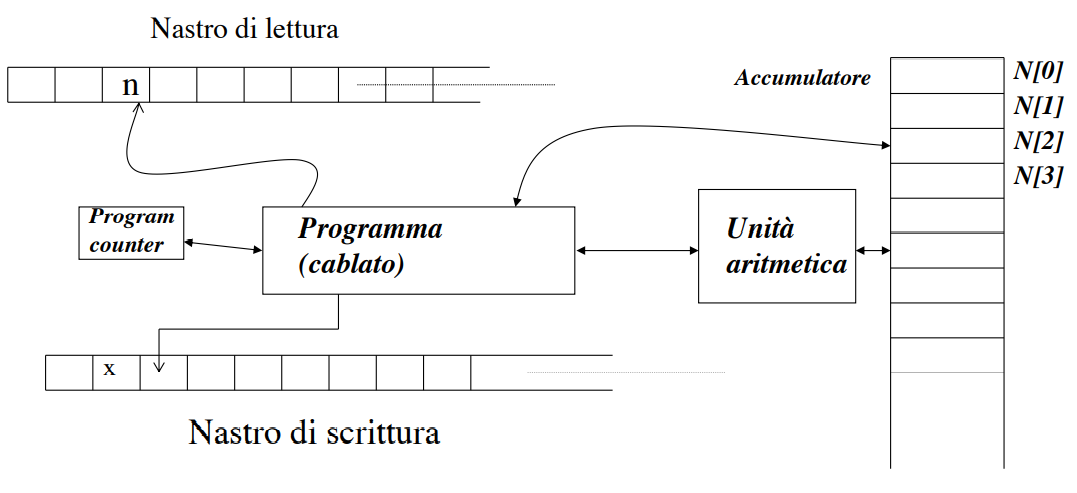
\includegraphics[width=\textwidth]{RAM.png}
  \end{figure}

  Sia i nastri che la memoria sono composti da un numero illimitato di celle, ma al contrario dei nastri di ingresso e uscita che si possono accedere in maniera sequenziale, la memoria è indirizzata e si può accedere a una sua cella attraverso un numero intero \(i>0\) che indica l'indirizzo di tale cella di memoria. La cella 0 della memoria è un registro speciale, detto accumulatore, che si utilizza per contenere il valore di uno dei due operandi delle operazioni aritmetiche binarie che la macchina può effettuare. Un generico programma eseguibile dalla macchina RAM è composto da istruzioni riportate nella tabella \ref{tabella istruzioni RAM}.

  \begin{table}[!h] 
    \caption{istruzioni macchina RAM}
    \vspace*{10pt}
    
    \centering
    \begin{tabular}{l l | l} \label{tabella istruzioni RAM}
      ISTRUZIONE & & SEMANTICA\\
      \hline
      LOAD= & \(x\) & M[0] \(\leftarrow x\)\\
      LOAD & \(x\)  & M[0] \(\leftarrow\) M[\(x\)]\\
      LOAD* & \(x\) & M[0] \(\leftarrow\) M[M[\(x\)]]\\
      STORE & \(x\) & M[\(x\)] \(\leftarrow\) M[0]\\
      STORE* & \(x\) & M[M[\(x\)]] \(\leftarrow\) M[0]\\
      ADD= & \(x\) & M[0] \(\leftarrow\) M[0] + \(x\)\\
      ADD  & \(x\)& M[0] \(\leftarrow\) M[0]+ M[\(x\)]\\
      ADD* & \(x\)& M[0] \(\leftarrow\) M[0] + M[M[\(x\)]]\\
      SUB= & \(x\)& M[0] \(\leftarrow\) M[0] - \(x\)\\
      SUB & \(x\)& M[0] \(\leftarrow\) M[0] - M[\(x\)]\\
      SUB* & \(x\)& M[0] \(\leftarrow\) M[0] - M[M[\(x\)]]\\
      MULT= & \(x\)& M[0] \(\leftarrow\) M[0] * \(x\)\\
      MULT & \(x\)& M[0] \(\leftarrow\) M[0] * M[\(x\)]\\
      MULT* & \(x\)& M[0] \(\leftarrow\) M[0] * M[M[0]]\\
      DIV= & \(x\)& M[0] \(\leftarrow\) M[0] \(\backslash\) \(x\) \\
      DIV & \(x\)& M[0] \(\leftarrow\) M[0] \(\backslash\) M[\(x\)]\\
      DIV* & \(x\)& M[0] \(\leftarrow\) M[0] \(\backslash\) M[M[\(x\)]]\\
      READ & \(x\)& M[x] \(\leftarrow\) input\\
      READ* & \(x\)& M[M[x]] \(\leftarrow\) input\\
      WRITE= & \(x\)& stampa \(x\)\\
      WRITE & \(x\)& stampa M[\(x\)]\\
      WRITE* & \(x\)& stampa M[M[\(x\)]]\\
      JUMP & \(label\)& PC \(\leftarrow\) \(label\) \\
      JGZ & \(label\)& PC \(\leftarrow\) \(label\) if M[0] \(>\) 0\\
      JLZ & \(label\)& PC \(\leftarrow\) \(label\) if M[0] \(<\) 0 \\
      JZ & \(label\)& PC \(\leftarrow\) \(label\) if M[0] = 0\\
      HALT & & terminazione\\
    \end{tabular}
  \end{table}

  Una volta introdotte tutte le istruzioni eseguibili dalla macchina RAM, è possibile ora studiarne la complessità temporale, come fatto per le TM a \(k\)-nastri. A differenza delle TM, nelle macchine RAM l'esecuzione delle diverse operazioni dipende dagli operandi necessari per eseguire tale operazione. Diventa quindi necessario analizzare tutte le istruzioni e definire il tempo richiesto per ciascuna di esse e la quantità di memoria allocata. Queste quantità possono essere calcolate secondo due criteri, ovvero tramite il criterio del costo costante e tramite il criterio del costo logaritmico. Il primo si basa sull'assunzione che l'esecuzione di ciascuna istruzione richieda un'unità di tempo e che ciascuna allocazione in memoria richieda un'unità di spazio (stessa assunzione fatta per le TM). 
  
  Si è appena affermato però che nella macchina RAM le istruzioni hanno diversa natura e manipolano dati di diversa dimensione: risulta, dunque, evidente che tale criterio è poco affine alla realtà. Per tener conto della differente velocità di esecuzione e della differente quantità di memoria allocata da ciascuna istruzione, si introduce il secondo criterio (del costo logaritmico), basato sulla supposizione che il tempo richiesto per eseguire un'istruzione sia proporzionale alla lunghezza degli operandi dell'istruzione considerata. Poichè gli operandi sono rappresentati in memoria in codice binario, un generico operando di valore \(v\) è rappresentato da \(\lfloor log_2(|v|+1)\rfloor\). 
  
  Dunque, è possibile definire la funzione \(l(i) = if\;i\neq 0\;then\;\lfloor log_2(|v|+1)\rfloor\;else\;1\) tramite cui calcolare la complessità temporale logaritmica di ciascuna istruzione precedentemente analizzata nella tabella \ref{tabella istruzioni RAM}. Alla stessa maniera, è possibile calcolare i costi relativi allo spazio, introducendo la variabile \(m\) definita come l'indirizzo più alto della cella di memoria a cui si fa accesso durante l'esecuzione del programma, e la variabile \(M_i\) che rappresenta il valore assoluto più grande immagazzinato in M[i] durante l'esecuzione. La complessità spaziale logaritmica si definisce quindi con la seguente formula:

  \(\displaystyle \sum_{i=0}^m{l(M_i)}\)\\
  Di seguito sono riportati i costi logaritmici delle istruzioni RAM:

  \begin{table}[!htb] \label{tabella costi logaritmici}
    \caption{costi logaritmici delle istruzioni macchina RAM}
    \vspace*{10pt}
    
    \centering
    \begin{tabular}{l l | l}
      ISTRUZIONE & & COSTO LOGARITMICO\\
      \hline
      LOAD= & \(x\) & \(l(x)\)\\
      LOAD & \(x\)  & \(l(x) + l(M[x])\) \\
      LOAD* & \(x\) & \(l(x) + l(M[x]) + l(M[M[x]])\)\\
      STORE & \(x\) & \(l(M[0]) + l(x)\)\\
      STORE* & \(x\) & \(l(M[0]) + l(x) + l(M[x])\)\\
      ADD= & \(x\) & \(l(M[0]) + l(x)\)\\
      ADD  & \(x\)& \(l(M[0]) + l(x) + l(M[x])\)\\
      ADD* & \(x\)& \(l(M[0]) + l(x) + l(M[x]) + l(M[M[x]])\)\\
      & & SUB, MULT, DIV definite come ADD.\\
      READ & \(x\)& \(l(input) + l(x)\)\\
      READ* & \(x\)& \(l(input) + l(x) + l(M[x])\)\\
      WRITE= & \(x\)& \(l(x)\)\\
      WRITE & \(x\)& \(l(x) + l(M[x])\)\\
      WRITE* & \(x\)& \(l(x) + l(M[x]) + l(M[M[x]])\)\\
      JUMP & \(label\)& 1 \\
      JGZ & \(label\)& \(l(M[0])\)\\
      JLZ & \(label\)& \(l(M[0])\) \\
      JZ & \(label\)& \(l(M[0])\)\\
      HALT & & 1\\
    \end{tabular}
  \end{table}
  
  Dunque, il criterio del costo costante si può applicare solo in situazioni in cui si prevede che ogni valore che comparirà durante l'esecuzione del programma occupi esattamente una cella di memoria, altrimenti si deve necessariamente applicare il criterio del costo logaritmico, che porta ad un calcolo più preciso della complessità.
  

  \section{Correlazione temporale fra TM e RAM}
  Una volta analizzato il comportamento della macchina RAM, è possibile studiarne la correlazione con le TM. Nello specifico, è possibile simulare una TM deterministica a \(k\) nastri attraverso una macchina RAM, nel seguente modo: innanzitutto, si considera la memoria della RAM come suddivisa in blocchi, tutti di dimensione \(k\), ad eccezione del blocco 0, che ha dimensione \(k+1\), in quanto memorizza lo stato della TM e le posizioni delle \(k\) testine. I successivi blocchi vengono impiegati per contenere i valori contenuti nelle successive posizioni di ciascuno dei \(k\) nastri di memoria della TM. Dunque, il valore rappresentato nella \(i\)-esima cella del \(j\)-esimo nastro della TM è contenuto nella locazione \(c+k\cdot j+i\) in cui \(c\) è una costante opportuna della memoria della macchina RAM. 
  Inoltre, per accedere al valore presente sotto la testina di lettura di un determinato nastro è prima necessario eseguire un accesso diretto al blocco 0, per poter trovare la posizione del nastro stesso. Poi, per eseguire la funzione di transizione \(\delta(q,i,s_1,...,s_k)\) e la funzione di uscita \(\eta(q,i,s_1,...,s_k)\), si richiedono un numero prefissato di accessi in memoria per ottenere \(q,i,s_1,...,s_n\), necessari per l'esecuzione di tali funzioni.

  Tutto ciò conduce al seguente teorema:

  \begin{theorem}
    Una TM multinastro con complessità temporale \(T_M\) può essere simulata da una macchina RAM con complessità temporale \(T_R = \Theta( T_M)\), secondo il criterio di costo uniforme, oppure \(T_R = \Theta( T_M \cdot log( T_M))\), secondo il criterio di costo logaritmico. 
  \end{theorem}

  Ovviamente è possibile anche simulare una macchina RAM tramite una macchina di Turing, ma tale costruzione è molto più complessa e richiede un'analisi approfondita. Si enuncia quindi solo il seguente teorema:

  \begin{theorem}
    Sia L il linguaggio riconosciuto da una macchina RAM di complessità temporale \({T}_R\) secondo il criterio del costo logaritmico. Se il programma RAM non utilizza le istruzioni \(MULT\) e \(DIV\), allora L può essere riconosciuto da un'opportuna TM multinastro, in un tempo \({T}_M=\Theta({T}_R^2)\). 
  \end{theorem}

  Si può quindi osservare come il legame tra \({T}_M\) e \({T}_R\) sia di tipo polinomiale, implicazione molto importante perchè suggerisce quale sia la classe di problemi trattabili nella pratica.
  \chapter{Algoritmi}
In questo capitolo si analizzano a fondo i principali algoritmi di ordinamento e i relativi tempi di esecuzione. Nello specifico, si utilizzerà come modello di riferimento la macchina RAM con un criterio di costo costante, come analizzato nei capitoli precedenti. Prima di proseguire nella trattazione è necessario dare una definizione generale di algoritmo:

\begin{definition}
  Un algoritmo è una procedura di calcolo ben definita che prende un certo valore, o un insieme di valori, in input e genera un valore, o un insieme di valori, in output. Dunque, un algoritmo è una serie di passi computazionali che trasformano l'input in output.
\end{definition}

Un algoritmo può anche essere visto come uno strumento per la risoluzione di un problema computazionale ben definito: sotto questo sguardo, un algoritmo si definisce corretto se, per ogni istanza di input, termina con l'output corretto. Se un algoritmo è corretto, allora risolve quel determinato problema computazionale. Esistono molti modi per poter specificare un determinato algoritmo: si può utilizzare la lingua italiana o inglese, ma anche un linguaggio di programmazione come C, C++, JAVA e Pascal, o ancora tramite uno pseudocodice.

\section{Pseudocodifica}
La pseudocodifica può avvenire in molti modi, ma nel seguito si utilizzerano le convenzioni qui riportate:
\begin{itemize}
  \item L'indentazione serve ad indicare la struttura a blocchi dello pesudocodice, in modo da comprendere quali istruzioni appartengono, per esempio, ad un ciclo for, a un ciclo while o ad un if-else statement. Non sono utilizzate le parentesi graffe o parole chiave come begin ed end in quanto appesantiscono la sintassi;
  \item I costrutti iterativi \code{while}, \code{for}, \code{repeat-until} e il costrutto condizionale \code{if-else} hanno interpretazioni simili a quelle dei comuni linguaggi di programmazione. Il contatore del ciclo mantiene il suo valore dopo la fine del ciclo, quindi il valore che ha provocato la terminazione del ciclo stesso. Inoltre, si utilizza la parola chiave \code{to} quando il ciclo \code{for} incrementa il valore del suo contatore ad ogni iterazione, mentre si utilizza la parola chiave \code{down to} nel caso la variabile venga decrementata;
  \item Le assegnazioni di un valore ad una certa variabile avviene con il simbolo \code{:=}, differente dall'operatore \code{=}, che invece indica l'eguaglianza di due valori all'interno di un costrutto \code{if};
  \item Per identificare un elemento appartenente ad un array, si utilizza la notazione con le parentesi quadre, al cui interno si indica l'indice dell'elemento a cui si vuole accedere: \code{array[i]}; Per indicare un intervallo di valori all'interno dell'array si utilizza la seguente sintassi: \code{array[i..j]}, con cui si indica la sottomatrice composta dagli elementi compresi fra \(i\) e \(j\); 
  \item I dati utilizzati sono tipicamente organizzati in oggetti, formati da attributi, a cui si accede tramite la notazione punto: \code{oggetto.proprietà}. Le variabili che rappresentano un determinato oggetto sono trattate come puntatori a tale oggetto. Un puntatore che non fa riferimento ad alcun oggetto è inizializzato con il valore \code{NIL};
  \item I parametri vengono passati ad una procedura per valore: la procedura chiamata riceve una sua copia dei parametri e, quindi, se a una di queste variabili è assegnato un nuovo valore, la modifica non è visibile dalla procedura chiamante. Nel caso venga passato come argomento un oggetto, viene copiato il puntatore a tale oggetto e quindi le modifiche sono visibili anche dalla procedura chiamante;
  \item L'istruzione \code{return} restituisce immediatamente il controllo al punto in cui la procedura chiamante ha effettuato la chiamata. Le istruzioni \code{return} possono anche ritornare un valore al chiamante;
  \item Gli operatori booleani \code{and} e \code{or} sono cortocircuitati. Ciò significa che nella valutazione dell'espressione \code{x and y}, si valuta prima se il valore di \code{x} sia falso, in quanto, se lo fosse, l'intera espressione sarebbe falsa e non avrebbe quindi alcun senso valutare il valore della variabile \code{y}. Al contrario, nella valutazione dell'espressione \code{x or y}, si verifica innanzitutto se il valore di \code{x} sia vero, in quanto, se lo fosse, l'intera espressione sarebbe vera e non avrebbe quindi alcun senso valutare il valore della variabile \code{y}.
\end{itemize}

Tramite queste regole è possibile definire un generico algoritmo.

\section{Insertion Sort}
Una classe di algoritmi molto studiati è quella riguardante l'ordinamento di un vettore, che consiste nella disposizione dei suoi elementi in ordine crescente.

\vspace{10pt}

Il primo algoritmo analizzato è l'\textbf{insertion sort}, che prende in input una sequenza di \(n\) numeri\\ \(<a_1, a_2, ...,a_n>\) e restituisce in output una permutazione \(<a_1', a_2',...,a_n'>\) tale che \(a_1'\le a_2' \le ... \le a_n'\).

Questo algoritmo ordina sul posto \footnote{L'algoritmo risistema gli elementi della sequenza all'interno dell'array avendo, in ogni istante, al più un numero finito di elementi memorizzati all'esterno dell'array: ciò permette di risparmiare memoria nel calcolatore.} gli elementi assumendo che la sequenza da ordinare sia inizialmente partizionata in una sottosequenza già ordinata, all'inizio composta da un unico elemento (il primo dell'array), e una sottosequenza ancora da ordinare. Ad ogni iterazione viene rimosso un elemento dalla sottosequenza non ordinata e inserita nella posizione corretta all'interno della sottosequenza già ordinata. 

In pseudocodice:

\lstinputlisting{../docs/insertion_sort.txt}

All'inizio di ogni iterazione del ciclo \code{for}, il cui indice è \(j\), la sottosequenza di elementi \code{A[1..j-1]} è la parte ordinata dell'array, mentre la sottosequenza \code{A[j+1..n]} è costituita da elementi ancora da ordinare.

\vspace{10pt}

Si analizza ora il tempo di esecuzione della procedura \code{insertion sort}: per ogni \(j=2,3,...,n\) in cui \(n\) = \code{A.length}, si indica con \(t_j\) il numero di volte che il test del ciclo \code{while} nella riga 5 viene eseguito per quel determinato valore di \(j\).



  
\end{document}
